%! BibTeX Compiler = biber
\documentclass{article}
\usepackage{xcolor}
\definecolor{BLUELINK}{HTML}{0645AD}
\definecolor{DARKBLUELINK}{HTML}{0B0080}
\definecolor{LIGHTBLUELINK}{HTML}{3366BB}
\definecolor{PURPLELINK}{HTML}{663366}
\PassOptionsToPackage{hyphens}{url}
\usepackage[colorlinks=false ]{hyperref}
% for linking between references, figures, TOC, etc in the pdf document
\hypersetup{colorlinks,
linkcolor=DARKBLUELINK,
anchorcolor=DARKBLUELINK,
citecolor=DARKBLUELINK,
filecolor=DARKBLUELINK,
menucolor=DARKBLUELINK,
urlcolor=BLUELINK
} % Color citation links in purple
\PassOptionsToPackage{unicode}{hyperref}
\PassOptionsToPackage{naturalnames}{hyperref}

\usepackage[margin=60pt]{geometry}
\usepackage{amssymb,amsfonts,amsmath,amsthm,mathtools}
\usepackage{lmodern}
\usepackage{bm,bbold}
\usepackage{verbatim}
\usepackage{float}
\usepackage{listings, enumerate, enumitem}
\usepackage[export]{adjustbox}
\usepackage{tabu}
\usepackage{longtable}
\tabulinesep=0.6mm
\newcommand\cellwidth{\TX@col@width}
\usepackage{hhline}
\setlength{\arrayrulewidth}{1.2pt}
\usepackage{multicol,multirow,array}
\usepackage{etoolbox}
\AtBeginEnvironment{tabu}{\footnotesize}
\usepackage{booktabs}

\usepackage{graphicx}
\graphicspath{{artworks/}}
\makeatletter
\def\input@path{{artworks/}}
\makeatother
\pdfstringdefDisableCommands{%
\renewcommand*{\bm}[1]{#1}%
% any other necessary redefinitions
}
\newcommand{\specialcell}[2][c]{%
    \begin{tabular}[#1]{@{}c@{}}#2\end{tabular}}

\usepackage{xfrac, nicefrac}
\usepackage[backend=biber,style=nature]{biblatex}
\addbibresource{codon_models.bib}
\pdfinclusioncopyfonts=1

\begin{document}
\part*{Supplementary materials}
\tableofcontents
 
\pagebreak

\section{Pipeline summary}
\label{subsec:method-summary}

\begin{center}
    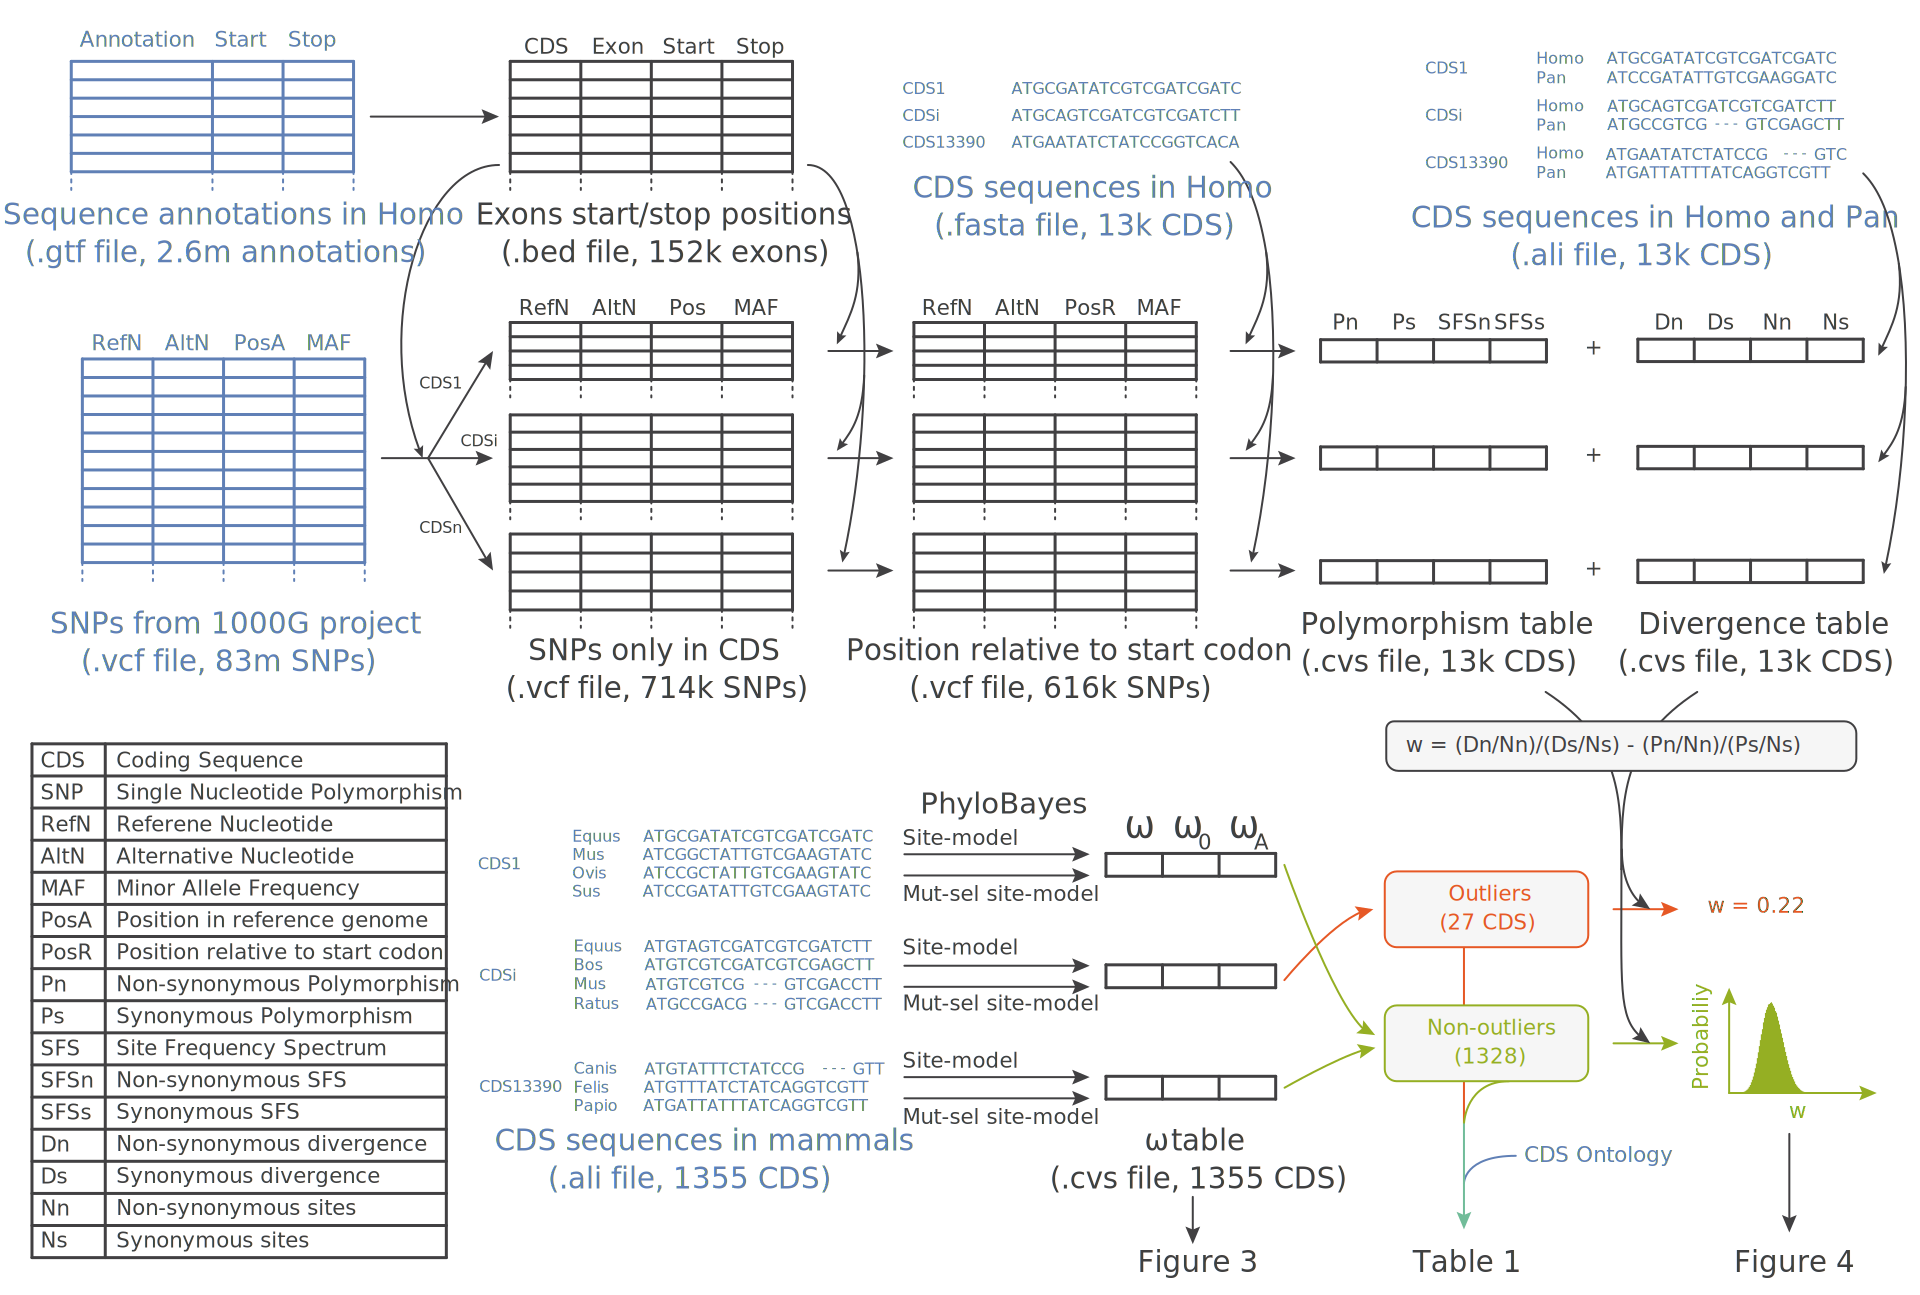
\includegraphics[width=\linewidth]{pipeline}
\end{center}

\pagebreak
\section{Rate of adaptation enrichment with $\alpha=0.005$}
\label{sec:threshold}
For each protein-coding DNA alignment, the Monte-Carlo Markov-Chain (MCMC) is run during $2000$ points using the \href{https://github.com/bayesiancook/bayescode}{BayesCode} software, after a burn-in of $1000$ points.
The mean of $\omega$ and $\omega_{0}$ are computed across the MCMC (after burn-in), as well as the $\bm{99.5}$\% confidence interval ($\alpha=0.005$) for each gene and site, which is more stringent than the $95$\% interval ($\alpha=0.05$) as shown in the main manuscript.
Genes and sites classified under an adaptive regime (in red) are rejecting the nearly-neutral assumption such that a lower bound for the confidence interval of $\omega$ is above the upper bound of the confidence interval of $\omega_{0}$, meaning $\omega > \omega_{0}$.
Genes and sites are classified under a nearly-neutral regime (in green) if the average $\omega$ is within the confidence interval of the $\omega_{0}$, and respectively the average $\omega_{0}$ is also within the confidence interval of  $\omega$, meaning $\omega = \omega_{0}$.
Genes and sites that do not fall in any of these categories are considered unclassified.

\subsection{Scatterplot with $\alpha=0.005$}

\begin{center}
    \begin{minipage}{0.32\linewidth}
        \includegraphics[width=\linewidth, page=1]{scatterplot-gene-MutSel-0.0025}
    \end{minipage}
    \llap{\raisebox{1.2cm}{\scriptsize A\hspace{4.7cm}}}\hfill
    \begin{minipage}{0.32\linewidth}
        \includegraphics[width=\linewidth, page=1]{scatterplot-site-MutSel-0.0025}
    \end{minipage}
    \llap{\raisebox{1.2cm}{\scriptsize B\hspace{4.7cm}}}\hfill
    \begin{minipage}{0.32\linewidth}
        \includegraphics[width=\linewidth, page=1]{scatterplot-site-MutSelExclu-0.0025}
    \end{minipage}
    \llap{\raisebox{1.2cm}{\scriptsize C\hspace{4.7cm}}}\hfill
\end{center}

$\omega$ estimated by the site model against $\omega_{0}$ calculated by the mutation-selection model.
Scatter plot of $14,509$ genes in panel A, with $99.5$\% confidence interval ($\alpha=0.005$).
Density plot of sites in panel B and C.
Genes or sites are then classified whether they detected as adaptive ($\omega > \omega_{0}$ in red) or nearly-neutral ($\omega \simeq \omega_{0}$ in green).
In panel C, the set of sites detected exclusively by mutation-selection codon models have a mean $\omega < 1 $.

\subsection{Folded SFS at gene level - grapes} 
\begin{center}
\includegraphics[width=\linewidth]{ViolinPlot/gene-folded-grapes.pdf} 
\begin{adjustbox}{width = 1\textwidth}
\begin{tabular}{llrrrrrrrrr}
\toprule
             Species &                Population & $\omega_{\textrm{A}}^{\textrm{S}}$ & $\omega_{\textrm{NA}}^{\textrm{S}}$ & $\omega^{\textrm{S}}$ & $\alpha^{\textrm{S}}$ & $\omega_{\textrm{A}}^{\textrm{N}}$ & $\omega_{\textrm{NA}}^{\textrm{N}}$ & $\omega^{\textrm{N}}$ & $\alpha^{\textrm{N}}$ &       p-value \\
\midrule
          Bos taurus &                      IRBT &                              0.126 &                               0.225 &                 0.351 &                 0.358 &                              0.163 &                               0.255 &                 0.418 &                 0.390 &         1.000 \\
          Bos taurus &                      UGBT &                              0.146 &                               0.206 &                 0.352 &                 0.414 &                              0.169 &                               0.252 &                 0.421 &                 0.401 &         1.000 \\
 Chlorocebus sabaeus &                  Barbados &                              0.237 &                               0.149 &                 0.386 &                 0.614 &                              0.142 &                               0.277 &                 0.419 &                 0.340 & 4.3e$^{-195}$ \\
 Chlorocebus sabaeus &  Central African Republic &                              0.169 &                               0.226 &                 0.395 &                 0.428 &                              0.157 &                               0.267 &                 0.424 &                 0.370 &   2.2e$^{-5}$ \\
 Chlorocebus sabaeus &                  Ethiopia &                              0.140 &                               0.256 &                 0.396 &                 0.353 &                              0.152 &                               0.273 &                 0.424 &                 0.358 &         1.000 \\
 Chlorocebus sabaeus &                    Gambia &                              0.160 &                               0.224 &                 0.384 &                 0.417 &                              0.121 &                               0.294 &                 0.416 &                 0.292 &  4.4e$^{-33}$ \\
 Chlorocebus sabaeus &                     Kenya &                              0.221 &                               0.180 &                 0.401 &                 0.552 &                              0.153 &                               0.276 &                 0.429 &                 0.356 &   5e$^{-152}$ \\
 Chlorocebus sabaeus &                     Nevis &                              0.153 &                               0.230 &                 0.384 &                 0.400 &                              0.111 &                               0.305 &                 0.416 &                 0.267 &  4.2e$^{-42}$ \\
 Chlorocebus sabaeus &               Saint Kitts &                              0.186 &                               0.197 &                 0.382 &                 0.486 &                              0.120 &                               0.294 &                 0.415 &                 0.290 &  9.1e$^{-88}$ \\
 Chlorocebus sabaeus &              South Africa &                              0.213 &                               0.176 &                 0.388 &                 0.548 &                              0.141 &                               0.278 &                 0.420 &                 0.337 & 5.4e$^{-142}$ \\
 Chlorocebus sabaeus &                    Zambia &                              0.217 &                               0.177 &                 0.395 &                 0.551 &                              0.154 &                               0.270 &                 0.424 &                 0.363 & 1.1e$^{-103}$ \\
        Homo sapiens &                       AFR &                              0.194 &                               0.272 &                 0.466 &                 0.416 &                              0.168 &                               0.351 &                 0.519 &                 0.322 &  2.8e$^{-14}$ \\
        Homo sapiens &                       AMR &                              0.168 &                               0.297 &                 0.465 &                 0.361 &                              0.129 &                               0.389 &                 0.518 &                 0.249 &  3.7e$^{-21}$ \\
        Homo sapiens &                       EAS &                              0.162 &                               0.303 &                 0.466 &                 0.349 &                              0.149 &                               0.370 &                 0.519 &                 0.286 &   1.8e$^{-5}$ \\
        Homo sapiens &                       EUR &                              0.167 &                               0.298 &                 0.465 &                 0.359 &                              0.140 &                               0.379 &                 0.519 &                 0.269 &    6e$^{-11}$ \\
        Homo sapiens &                       SAS &                              0.200 &                               0.265 &                 0.465 &                 0.430 &                              0.122 &                               0.397 &                 0.519 &                 0.235 &  1.4e$^{-67}$ \\
          Ovis aries &                      IROA &                              0.233 &                               0.120 &                 0.353 &                 0.659 &                              0.178 &                               0.220 &                 0.397 &                 0.447 &  1.1e$^{-80}$ \\
          Ovis aries &                      IROO &                              0.248 &                               0.106 &                 0.353 &                 0.701 &                              0.175 &                               0.223 &                 0.398 &                 0.439 &   3e$^{-134}$ \\
          Ovis aries &                      ISGC &                              0.243 &                               0.109 &                 0.352 &                 0.690 &                              0.173 &                               0.224 &                 0.396 &                 0.435 & 1.2e$^{-104}$ \\
\bottomrule
\end{tabular}
\end{adjustbox}
\end{center}
\subsection{Folded SFS at site level - grapes} 
\begin{center}
\includegraphics[width=\linewidth]{ViolinPlot/site-folded-grapes.pdf} 
\begin{adjustbox}{width = 1\textwidth}
\begin{tabular}{llrrrrrrrrr}
\toprule
             Species &                Population & $\omega_{\textrm{A}}^{\textrm{S}}$ & $\omega_{\textrm{NA}}^{\textrm{S}}$ & $\omega^{\textrm{S}}$ & $\alpha^{\textrm{S}}$ & $\omega_{\textrm{A}}^{\textrm{N}}$ & $\omega_{\textrm{NA}}^{\textrm{N}}$ & $\omega^{\textrm{N}}$ & $\alpha^{\textrm{N}}$ &       p-value \\
\midrule
          Bos taurus &                      IRBT &                              0.276 &                               0.376 &                 0.652 &                 0.423 &                              0.225 &                               0.438 &                 0.663 &                 0.338 &  6.6e$^{-62}$ \\
          Bos taurus &                      UGBT &                              0.325 &                               0.331 &                 0.656 &                 0.495 &                              0.188 &                               0.477 &                 0.665 &                 0.281 & 1.5e$^{-193}$ \\
 Chlorocebus sabaeus &                  Barbados &                              0.531 &                               0.163 &                 0.694 &                 0.765 &                              0.216 &                               0.462 &                 0.678 &                 0.318 & 1.1e$^{-267}$ \\
 Chlorocebus sabaeus &  Central African Republic &                              0.279 &                               0.424 &                 0.702 &                 0.396 &                              0.178 &                               0.505 &                 0.683 &                 0.259 & 1.2e$^{-116}$ \\
 Chlorocebus sabaeus &                  Ethiopia &                              0.358 &                               0.340 &                 0.698 &                 0.513 &                              0.181 &                               0.501 &                 0.682 &                 0.264 & 6.6e$^{-181}$ \\
 Chlorocebus sabaeus &                    Gambia &                              0.355 &                               0.340 &                 0.695 &                 0.510 &                              0.187 &                               0.492 &                 0.678 &                 0.275 &   3e$^{-158}$ \\
 Chlorocebus sabaeus &                     Kenya &                              0.286 &                               0.416 &                 0.702 &                 0.407 &                              0.144 &                               0.543 &                 0.688 &                 0.209 & 2.3e$^{-234}$ \\
 Chlorocebus sabaeus &                     Nevis &                              0.236 &                               0.459 &                 0.695 &                 0.338 &                              0.184 &                               0.495 &                 0.679 &                 0.269 &  2.7e$^{-47}$ \\
 Chlorocebus sabaeus &               Saint Kitts &                              0.250 &                               0.446 &                 0.695 &                 0.358 &                              0.127 &                               0.550 &                 0.677 &                 0.186 & 2.2e$^{-209}$ \\
 Chlorocebus sabaeus &              South Africa &                              0.245 &                               0.454 &                 0.699 &                 0.349 &                              0.212 &                               0.468 &                 0.680 &                 0.310 &    2e$^{-15}$ \\
 Chlorocebus sabaeus &                    Zambia &                              0.211 &                               0.489 &                 0.700 &                 0.300 &                              0.235 &                               0.450 &                 0.685 &                 0.343 &         1.000 \\
        Homo sapiens &                       AFR &                              0.288 &                               0.442 &                 0.729 &                 0.394 &                              0.312 &                               0.478 &                 0.790 &                 0.394 &         0.998 \\
        Homo sapiens &                       AMR &                              0.297 &                               0.432 &                 0.729 &                 0.407 &                              0.317 &                               0.473 &                 0.790 &                 0.401 &         0.991 \\
        Homo sapiens &                       EAS &                              0.334 &                               0.396 &                 0.730 &                 0.458 &                              0.296 &                               0.495 &                 0.791 &                 0.373 &    8e$^{-10}$ \\
        Homo sapiens &                       EUR &                              0.285 &                               0.445 &                 0.730 &                 0.390 &                              0.283 &                               0.507 &                 0.790 &                 0.358 &         0.235 \\
        Homo sapiens &                       SAS &                              0.286 &                               0.443 &                 0.729 &                 0.392 &                              0.298 &                               0.492 &                 0.790 &                 0.377 &         0.890 \\
          Ovis aries &                      IROA &                              0.342 &                               0.282 &                 0.624 &                 0.548 &                              0.200 &                               0.453 &                 0.652 &                 0.306 & 1.1e$^{-176}$ \\
          Ovis aries &                      IROO &                              0.394 &                               0.231 &                 0.625 &                 0.630 &                              0.217 &                               0.437 &                 0.654 &                 0.331 & 1.2e$^{-201}$ \\
          Ovis aries &                      ISGC &                              0.368 &                               0.257 &                 0.625 &                 0.588 &                              0.223 &                               0.428 &                 0.652 &                 0.343 & 1.4e$^{-161}$ \\
\bottomrule
\end{tabular}
\end{adjustbox}
\end{center}
\subsection{Unfolded SFS at gene level - grapes} 
\begin{center}
\includegraphics[width=\linewidth]{ViolinPlot/gene-unfolded-grapes.pdf} 
\begin{adjustbox}{width = 1\textwidth}
\begin{tabular}{llrrrrrrrrr}
\toprule
             Species &                Population & $\omega_{\textrm{A}}^{\textrm{S}}$ & $\omega_{\textrm{NA}}^{\textrm{S}}$ & $\omega^{\textrm{S}}$ & $\alpha^{\textrm{S}}$ & $\omega_{\textrm{A}}^{\textrm{N}}$ & $\omega_{\textrm{NA}}^{\textrm{N}}$ & $\omega^{\textrm{N}}$ & $\alpha^{\textrm{N}}$ &       p-value \\
\midrule
          Bos taurus &                      IRBT &                              0.120 &                               0.273 &                 0.393 &                 0.305 &                              0.189 &                               0.276 &                 0.465 &                 0.406 &         1.000 \\
          Bos taurus &                      UGBT &                              0.130 &                               0.267 &                 0.397 &                 0.327 &                              0.168 &                               0.298 &                 0.466 &                 0.359 &         1.000 \\
 Chlorocebus sabaeus &                  Barbados &                              0.190 &                               0.206 &                 0.395 &                 0.479 &                              0.076 &                               0.352 &                 0.429 &                 0.178 & 2.7e$^{-267}$ \\
 Chlorocebus sabaeus &  Central African Republic &                              0.186 &                               0.221 &                 0.407 &                 0.456 &                              0.088 &                               0.349 &                 0.436 &                 0.201 & 1.4e$^{-249}$ \\
 Chlorocebus sabaeus &                  Ethiopia &                              0.084 &                               0.322 &                 0.406 &                 0.207 &                              0.084 &                               0.352 &                 0.436 &                 0.192 &         1.000 \\
 Chlorocebus sabaeus &                    Gambia &                              0.094 &                               0.305 &                 0.399 &                 0.236 &                              0.139 &                               0.294 &                 0.433 &                 0.322 &         1.000 \\
 Chlorocebus sabaeus &                     Kenya &                              0.206 &                               0.202 &                 0.407 &                 0.505 &                              0.080 &                               0.357 &                 0.437 &                 0.183 & 4.3e$^{-293}$ \\
 Chlorocebus sabaeus &                     Nevis &                              0.082 &                               0.313 &                 0.395 &                 0.208 &                              0.052 &                               0.376 &                 0.429 &                 0.122 &  3.6e$^{-47}$ \\
 Chlorocebus sabaeus &               Saint Kitts &                              0.108 &                               0.289 &                 0.398 &                 0.272 &                              0.081 &                               0.350 &                 0.431 &                 0.189 &  1.5e$^{-34}$ \\
 Chlorocebus sabaeus &              South Africa &                              0.162 &                               0.243 &                 0.405 &                 0.400 &                              0.115 &                               0.322 &                 0.437 &                 0.264 &  1.1e$^{-64}$ \\
 Chlorocebus sabaeus &                    Zambia &                              0.154 &                               0.252 &                 0.406 &                 0.380 &                              0.103 &                               0.335 &                 0.438 &                 0.235 &  3.9e$^{-71}$ \\
        Homo sapiens &                       AFR &                              0.204 &                               0.280 &                 0.484 &                 0.420 &                              0.175 &                               0.361 &                 0.535 &                 0.326 &  1.7e$^{-17}$ \\
        Homo sapiens &                       AMR &                              0.119 &                               0.364 &                 0.483 &                 0.246 &                              0.132 &                               0.400 &                 0.532 &                 0.247 &         1.000 \\
        Homo sapiens &                       EAS &                              0.126 &                               0.355 &                 0.481 &                 0.261 &                              0.156 &                               0.377 &                 0.532 &                 0.292 &         1.000 \\
        Homo sapiens &                       EUR &                              0.121 &                               0.360 &                 0.481 &                 0.252 &                              0.139 &                               0.394 &                 0.532 &                 0.260 &         1.000 \\
        Homo sapiens &                       SAS &                              0.163 &                               0.319 &                 0.482 &                 0.338 &                              0.129 &                               0.405 &                 0.533 &                 0.241 &  2.4e$^{-21}$ \\
          Ovis aries &                      IROA &                              0.204 &                               0.162 &                 0.366 &                 0.557 &                              0.135 &                               0.277 &                 0.413 &                 0.328 & 6.5e$^{-195}$ \\
          Ovis aries &                      IROO &                              0.230 &                               0.138 &                 0.368 &                 0.625 &                              0.130 &                               0.285 &                 0.416 &                 0.314 & 8.7e$^{-248}$ \\
          Ovis aries &                      ISGC &                              0.217 &                               0.151 &                 0.368 &                 0.590 &                              0.122 &                               0.292 &                 0.415 &                 0.295 & 4.9e$^{-254}$ \\
\bottomrule
\end{tabular}
\end{adjustbox}
\end{center}
\subsection{Unfolded SFS at gene level - polyDFE} 
\begin{center}
\includegraphics[width=\linewidth]{ViolinPlot/gene-unfolded-polyDFE.pdf} 
\begin{adjustbox}{width = 1\textwidth}
\begin{tabular}{llrrrrrrrrr}
\toprule
             Species &                Population & $\omega_{\textrm{A}}^{\textrm{S}}$ & $\omega_{\textrm{NA}}^{\textrm{S}}$ & $\omega^{\textrm{S}}$ & $\alpha^{\textrm{S}}$ & $\omega_{\textrm{A}}^{\textrm{N}}$ & $\omega_{\textrm{NA}}^{\textrm{N}}$ & $\omega^{\textrm{N}}$ & $\alpha^{\textrm{N}}$ &       p-value \\
\midrule
          Bos taurus &                      IRBT &                              0.384 &                               0.009 &                 0.393 &                 0.977 &                              0.190 &                               0.275 &                 0.465 &                 0.409 & 7.9e$^{-295}$ \\
          Bos taurus &                      UGBT &                              0.362 &                               0.035 &                 0.397 &                 0.912 &                              0.175 &                               0.291 &                 0.466 &                 0.376 & 5.2e$^{-265}$ \\
 Chlorocebus sabaeus &                  Barbados &                              0.231 &                               0.165 &                 0.396 &                 0.583 &                              0.158 &                               0.271 &                 0.429 &                 0.368 &  1.9e$^{-89}$ \\
 Chlorocebus sabaeus &  Central African Republic &                              0.357 &                               0.050 &                 0.407 &                 0.877 &                              0.194 &                               0.243 &                 0.436 &                 0.444 & 4.6e$^{-124}$ \\
 Chlorocebus sabaeus &                  Ethiopia &                              0.333 &                               0.073 &                 0.406 &                 0.821 &                              0.085 &                               0.351 &                 0.436 &                 0.195 & 2.8e$^{-262}$ \\
 Chlorocebus sabaeus &                    Gambia &                              0.317 &                               0.083 &                 0.399 &                 0.792 &                              0.122 &                               0.311 &                 0.433 &                 0.282 & 4.9e$^{-277}$ \\
 Chlorocebus sabaeus &                     Kenya &                              0.212 &                               0.195 &                 0.407 &                 0.521 &                              0.168 &                               0.268 &                 0.437 &                 0.385 &  1.9e$^{-83}$ \\
 Chlorocebus sabaeus &                     Nevis &                              0.124 &                               0.271 &                 0.395 &                 0.314 &                              0.076 &                               0.352 &                 0.428 &                 0.177 & 5.8e$^{-180}$ \\
 Chlorocebus sabaeus &               Saint Kitts &                              0.186 &                               0.212 &                 0.398 &                 0.468 &                              0.073 &                               0.357 &                 0.430 &                 0.169 &   1e$^{-249}$ \\
 Chlorocebus sabaeus &              South Africa &                              0.278 &                               0.126 &                 0.405 &                 0.687 &                              0.095 &                               0.342 &                 0.437 &                 0.217 &             0 \\
 Chlorocebus sabaeus &                    Zambia &                              0.259 &                               0.147 &                 0.406 &                 0.637 &                              0.127 &                               0.311 &                 0.438 &                 0.290 & 3.9e$^{-198}$ \\
        Homo sapiens &                       AFR &                              0.222 &                               0.262 &                 0.484 &                 0.459 &                              0.272 &                               0.263 &                 0.535 &                 0.508 &         0.929 \\
        Homo sapiens &                       AMR &                              0.150 &                               0.333 &                 0.483 &                 0.310 &                              0.242 &                               0.290 &                 0.532 &                 0.455 &         1.000 \\
        Homo sapiens &                       EAS &                              0.117 &                               0.365 &                 0.481 &                 0.242 &                              0.197 &                               0.335 &                 0.532 &                 0.370 &         1.000 \\
        Homo sapiens &                       EUR &                              0.144 &                               0.337 &                 0.481 &                 0.299 &                              0.263 &                               0.269 &                 0.532 &                 0.494 &         1.000 \\
        Homo sapiens &                       SAS &                              0.191 &                               0.291 &                 0.482 &                 0.394 &                              0.223 &                               0.311 &                 0.534 &                 0.417 &         0.004 \\
          Ovis aries &                      IROA &                              0.299 &                               0.067 &                 0.366 &                 0.817 &                              0.141 &                               0.272 &                 0.413 &                 0.342 & 6.3e$^{-288}$ \\
          Ovis aries &                      IROO &                              0.299 &                               0.069 &                 0.368 &                 0.811 &                              0.172 &                               0.243 &                 0.416 &                 0.414 & 5.7e$^{-181}$ \\
          Ovis aries &                      ISGC &                              0.293 &                               0.076 &                 0.368 &                 0.795 &                              0.148 &                               0.266 &                 0.415 &                 0.358 & 1.3e$^{-233}$ \\
\bottomrule
\end{tabular}
\end{adjustbox}
\end{center}
\subsection{Unfolded SFS at gene level - MK} 
\begin{center}
\includegraphics[width=\linewidth]{ViolinPlot/gene-unfolded-MK.pdf} 
\begin{adjustbox}{width = 1\textwidth}
\begin{tabular}{llrrrrrrrrr}
\toprule
             Species &                Population & $\omega_{\textrm{A}}^{\textrm{S}}$ & $\omega_{\textrm{NA}}^{\textrm{S}}$ & $\omega^{\textrm{S}}$ & $\alpha^{\textrm{S}}$ & $\omega_{\textrm{A}}^{\textrm{N}}$ & $\omega_{\textrm{NA}}^{\textrm{N}}$ & $\omega^{\textrm{N}}$ & $\alpha^{\textrm{N}}$ &       p-value \\
\midrule
          Bos taurus &                      IRBT &                              0.142 &                               0.252 &                 0.393 &                 0.360 &                              0.109 &                               0.356 &                 0.465 &                 0.234 & 1.5e$^{-285}$ \\
          Bos taurus &                      UGBT &                              0.143 &                               0.253 &                 0.397 &                 0.361 &                              0.112 &                               0.354 &                 0.466 &                 0.240 &   2e$^{-271}$ \\
 Chlorocebus sabaeus &                  Barbados &                              0.106 &                               0.290 &                 0.395 &                 0.267 &                              0.018 &                               0.411 &                 0.429 &                 0.042 &             0 \\
 Chlorocebus sabaeus &  Central African Republic &                              0.096 &                               0.311 &                 0.407 &                 0.236 &                              0.045 &                               0.392 &                 0.436 &                 0.102 &             0 \\
 Chlorocebus sabaeus &                  Ethiopia &                              0.061 &                               0.345 &                 0.406 &                 0.150 &                              0.007 &                               0.429 &                 0.436 &                 0.017 &             0 \\
 Chlorocebus sabaeus &                    Gambia &                              0.077 &                               0.322 &                 0.400 &                 0.193 &                              0.029 &                               0.404 &                 0.433 &                 0.067 & 5.5e$^{-310}$ \\
 Chlorocebus sabaeus &                     Kenya &                              0.101 &                               0.307 &                 0.407 &                 0.247 &                              0.046 &                               0.390 &                 0.437 &                 0.105 &             0 \\
 Chlorocebus sabaeus &                     Nevis &                              0.055 &                               0.340 &                 0.395 &                 0.139 &                              0.006 &                               0.422 &                 0.428 &                 0.014 & 7.9e$^{-288}$ \\
 Chlorocebus sabaeus &               Saint Kitts &                              0.066 &                               0.332 &                 0.398 &                 0.166 &                              0.010 &                               0.420 &                 0.430 &                 0.024 &             0 \\
 Chlorocebus sabaeus &              South Africa &                              0.092 &                               0.312 &                 0.405 &                 0.228 &                              0.025 &                               0.413 &                 0.437 &                 0.056 &             0 \\
 Chlorocebus sabaeus &                    Zambia &                              0.096 &                               0.311 &                 0.406 &                 0.236 &                              0.019 &                               0.419 &                 0.438 &                 0.044 &             0 \\
        Homo sapiens &                       AFR &                              0.048 &                               0.436 &                 0.484 &                 0.099 &                              0.009 &                               0.526 &                 0.535 &                 0.017 & 1.9e$^{-164}$ \\
        Homo sapiens &                       AMR &                              0.036 &                               0.448 &                 0.483 &                 0.073 &                             -0.014 &                               0.545 &                 0.532 &                -0.026 & 4.2e$^{-197}$ \\
        Homo sapiens &                       EAS &                              0.023 &                               0.459 &                 0.481 &                 0.047 &                             -0.010 &                               0.542 &                 0.532 &                -0.019 & 3.7e$^{-101}$ \\
        Homo sapiens &                       EUR &                              0.031 &                               0.451 &                 0.481 &                 0.063 &                             -0.019 &                               0.552 &                 0.532 &                -0.037 & 1.1e$^{-199}$ \\
        Homo sapiens &                       SAS &                              0.047 &                               0.435 &                 0.482 &                 0.098 &                             -0.024 &                               0.557 &                 0.534 &                -0.045 & 7.2e$^{-279}$ \\
          Ovis aries &                      IROA &                              0.173 &                               0.193 &                 0.366 &                 0.472 &                              0.078 &                               0.335 &                 0.413 &                 0.189 &             0 \\
          Ovis aries &                      IROO &                              0.174 &                               0.195 &                 0.368 &                 0.471 &                              0.079 &                               0.337 &                 0.416 &                 0.190 &             0 \\
          Ovis aries &                      ISGC &                              0.172 &                               0.196 &                 0.368 &                 0.467 &                              0.079 &                               0.335 &                 0.415 &                 0.191 &             0 \\
\bottomrule
\end{tabular}
\end{adjustbox}
\end{center}
\subsection{Unfolded SFS at site level - grapes} 
\begin{center}
\includegraphics[width=\linewidth]{ViolinPlot/site-unfolded-grapes.pdf} 
\begin{adjustbox}{width = 1\textwidth}
\begin{tabular}{llrrrrrrrrr}
\toprule
             Species &                Population & $\omega_{\textrm{A}}^{\textrm{S}}$ & $\omega_{\textrm{NA}}^{\textrm{S}}$ & $\omega^{\textrm{S}}$ & $\alpha^{\textrm{S}}$ & $\omega_{\textrm{A}}^{\textrm{N}}$ & $\omega_{\textrm{NA}}^{\textrm{N}}$ & $\omega^{\textrm{N}}$ & $\alpha^{\textrm{N}}$ &       p-value \\
\midrule
          Bos taurus &                      IRBT &                              0.250 &                               0.420 &                 0.670 &                 0.372 &                              0.255 &                               0.441 &                 0.697 &                 0.365 &         0.597 \\
          Bos taurus &                      UGBT &                              0.300 &                               0.368 &                 0.668 &                 0.448 &                              0.195 &                               0.505 &                 0.699 &                 0.277 & 3.3e$^{-147}$ \\
 Chlorocebus sabaeus &                  Barbados &                              0.533 &                               0.172 &                 0.705 &                 0.756 &                              0.223 &                               0.464 &                 0.687 &                 0.324 &   3e$^{-291}$ \\
 Chlorocebus sabaeus &  Central African Republic &                              0.249 &                               0.456 &                 0.706 &                 0.353 &                              0.155 &                               0.534 &                 0.690 &                 0.224 & 6.6e$^{-109}$ \\
 Chlorocebus sabaeus &                  Ethiopia &                              0.370 &                               0.336 &                 0.706 &                 0.524 &                              0.159 &                               0.531 &                 0.690 &                 0.229 & 1.8e$^{-242}$ \\
 Chlorocebus sabaeus &                    Gambia &                              0.372 &                               0.335 &                 0.707 &                 0.525 &                              0.160 &                               0.529 &                 0.689 &                 0.231 & 3.4e$^{-209}$ \\
 Chlorocebus sabaeus &                     Kenya &                              0.264 &                               0.445 &                 0.708 &                 0.371 &                              0.126 &                               0.566 &                 0.692 &                 0.182 & 6.6e$^{-186}$ \\
 Chlorocebus sabaeus &                     Nevis &                              0.181 &                               0.522 &                 0.703 &                 0.257 &                              0.152 &                               0.533 &                 0.684 &                 0.220 &  1.2e$^{-19}$ \\
 Chlorocebus sabaeus &               Saint Kitts &                              0.193 &                               0.515 &                 0.708 &                 0.272 &                              0.092 &                               0.596 &                 0.688 &                 0.132 & 5.1e$^{-131}$ \\
 Chlorocebus sabaeus &              South Africa &                              0.217 &                               0.495 &                 0.712 &                 0.304 &                              0.194 &                               0.496 &                 0.690 &                 0.281 &   3.6e$^{-8}$ \\
 Chlorocebus sabaeus &                    Zambia &                              0.180 &                               0.528 &                 0.709 &                 0.254 &                              0.199 &                               0.491 &                 0.690 &                 0.288 &         0.981 \\
        Homo sapiens &                       AFR &                              0.230 &                               0.501 &                 0.731 &                 0.314 &                              0.290 &                               0.509 &                 0.799 &                 0.362 &         1.000 \\
        Homo sapiens &                       AMR &                              0.207 &                               0.524 &                 0.732 &                 0.282 &                              0.307 &                               0.489 &                 0.796 &                 0.385 &         1.000 \\
        Homo sapiens &                       EAS &                              0.253 &                               0.478 &                 0.731 &                 0.346 &                              0.287 &                               0.512 &                 0.799 &                 0.358 &         1.000 \\
        Homo sapiens &                       EUR &                              0.259 &                               0.472 &                 0.731 &                 0.355 &                              0.282 &                               0.516 &                 0.797 &                 0.353 &         0.996 \\
        Homo sapiens &                       SAS &                              0.266 &                               0.464 &                 0.730 &                 0.364 &                              0.279 &                               0.519 &                 0.798 &                 0.349 &         0.907 \\
          Ovis aries &                      IROA &                              0.282 &                               0.343 &                 0.625 &                 0.451 &                              0.175 &                               0.492 &                 0.667 &                 0.262 & 1.4e$^{-140}$ \\
          Ovis aries &                      IROO &                              0.323 &                               0.301 &                 0.625 &                 0.517 &                              0.199 &                               0.470 &                 0.670 &                 0.297 & 7.8e$^{-161}$ \\
          Ovis aries &                      ISGC &                              0.306 &                               0.321 &                 0.627 &                 0.487 &                              0.204 &                               0.465 &                 0.669 &                 0.305 & 7.1e$^{-120}$ \\
\bottomrule
\end{tabular}
\end{adjustbox}
\end{center}
\subsection{Unfolded SFS at site level - polyDFE} 
\begin{center}
\includegraphics[width=\linewidth]{ViolinPlot/site-unfolded-polyDFE.pdf} 
\begin{adjustbox}{width = 1\textwidth}
\begin{tabular}{llrrrrrrrrr}
\toprule
             Species &                Population & $\omega_{\textrm{A}}^{\textrm{S}}$ & $\omega_{\textrm{NA}}^{\textrm{S}}$ & $\omega^{\textrm{S}}$ & $\alpha^{\textrm{S}}$ & $\omega_{\textrm{A}}^{\textrm{N}}$ & $\omega_{\textrm{NA}}^{\textrm{N}}$ & $\omega^{\textrm{N}}$ & $\alpha^{\textrm{N}}$ &       p-value \\
\midrule
          Bos taurus &                      IRBT &                              0.524 &                               0.145 &                 0.670 &                 0.782 &                              0.282 &                               0.415 &                 0.697 &                 0.403 & 1.5e$^{-150}$ \\
          Bos taurus &                      UGBT &                              0.401 &                               0.267 &                 0.668 &                 0.600 &                              0.221 &                               0.479 &                 0.699 &                 0.314 & 4.4e$^{-146}$ \\
 Chlorocebus sabaeus &                  Barbados &                              0.567 &                               0.137 &                 0.705 &                 0.805 &                              0.361 &                               0.326 &                 0.687 &                 0.526 &  3.3e$^{-93}$ \\
 Chlorocebus sabaeus &  Central African Republic &                              0.330 &                               0.376 &                 0.706 &                 0.466 &                              0.185 &                               0.505 &                 0.690 &                 0.267 &    4e$^{-88}$ \\
 Chlorocebus sabaeus &                  Ethiopia &                              0.519 &                               0.187 &                 0.706 &                 0.735 &                              0.235 &                               0.455 &                 0.690 &                 0.340 & 5.7e$^{-160}$ \\
 Chlorocebus sabaeus &                    Gambia &                              0.433 &                               0.274 &                 0.707 &                 0.612 &                              0.194 &                               0.495 &                 0.689 &                 0.281 & 1.7e$^{-145}$ \\
 Chlorocebus sabaeus &                     Kenya &                              0.344 &                               0.365 &                 0.708 &                 0.484 &                              0.553 &                               0.139 &                 0.692 &                 0.799 &         1.000 \\
 Chlorocebus sabaeus &                     Nevis &                              0.368 &                               0.335 &                 0.703 &                 0.523 &                              0.255 &                               0.429 &                 0.684 &                 0.372 &  6.3e$^{-36}$ \\
 Chlorocebus sabaeus &               Saint Kitts &                              0.327 &                               0.381 &                 0.708 &                 0.461 &                              0.197 &                               0.491 &                 0.688 &                 0.285 &  3.3e$^{-60}$ \\
 Chlorocebus sabaeus &              South Africa &                              0.213 &                               0.499 &                 0.712 &                 0.298 &                              0.215 &                               0.475 &                 0.690 &                 0.311 &   3.6e$^{-9}$ \\
 Chlorocebus sabaeus &                    Zambia &                              0.191 &                               0.517 &                 0.709 &                 0.269 &                              0.192 &                               0.498 &                 0.690 &                 0.277 &         0.541 \\
        Homo sapiens &                       AFR &                              0.217 &                               0.514 &                 0.731 &                 0.295 &                              0.326 &                               0.473 &                 0.799 &                 0.408 &         1.000 \\
        Homo sapiens &                       AMR &                              0.211 &                               0.521 &                 0.732 &                 0.287 &                              0.300 &                               0.497 &                 0.797 &                 0.374 &         1.000 \\
        Homo sapiens &                       EAS &                              0.213 &                               0.518 &                 0.731 &                 0.290 &                              0.301 &                               0.498 &                 0.799 &                 0.376 &         1.000 \\
        Homo sapiens &                       EUR &                              0.177 &                               0.554 &                 0.731 &                 0.242 &                              0.267 &                               0.532 &                 0.798 &                 0.333 &         1.000 \\
        Homo sapiens &                       SAS &                              0.143 &                               0.587 &                 0.730 &                 0.194 &                              0.285 &                               0.512 &                 0.797 &                 0.357 &         1.000 \\
          Ovis aries &                      IROA &                              0.363 &                               0.262 &                 0.625 &                 0.581 &                              0.209 &                               0.459 &                 0.667 &                 0.312 & 4.9e$^{-135}$ \\
          Ovis aries &                      IROO &                              0.374 &                               0.250 &                 0.625 &                 0.599 &                              0.197 &                               0.473 &                 0.670 &                 0.294 & 5.6e$^{-190}$ \\
          Ovis aries &                      ISGC &                              0.347 &                               0.280 &                 0.627 &                 0.553 &                              0.227 &                               0.441 &                 0.669 &                 0.339 & 5.6e$^{-118}$ \\
\bottomrule
\end{tabular}
\end{adjustbox}
\end{center}
\subsection{Unfolded SFS at site level - MK} 
\begin{center}
\includegraphics[width=\linewidth]{ViolinPlot/site-unfolded-MK.pdf} 
\begin{adjustbox}{width = 1\textwidth}
\begin{tabular}{llrrrrrrrrr}
\toprule
             Species &                Population & $\omega_{\textrm{A}}^{\textrm{S}}$ & $\omega_{\textrm{NA}}^{\textrm{S}}$ & $\omega^{\textrm{S}}$ & $\alpha^{\textrm{S}}$ & $\omega_{\textrm{A}}^{\textrm{N}}$ & $\omega_{\textrm{NA}}^{\textrm{N}}$ & $\omega^{\textrm{N}}$ & $\alpha^{\textrm{N}}$ &       p-value \\
\midrule
          Bos taurus &                      IRBT &                              0.194 &                               0.476 &                 0.670 &                 0.288 &                              0.065 &                               0.632 &                 0.697 &                 0.091 &             0 \\
          Bos taurus &                      UGBT &                              0.204 &                               0.464 &                 0.668 &                 0.304 &                              0.061 &                               0.638 &                 0.699 &                 0.086 &             0 \\
 Chlorocebus sabaeus &                  Barbados &                              0.210 &                               0.495 &                 0.705 &                 0.297 &                             -0.041 &                               0.728 &                 0.687 &                -0.061 &             0 \\
 Chlorocebus sabaeus &  Central African Republic &                              0.102 &                               0.604 &                 0.706 &                 0.144 &                           -0.00019 &                               0.690 &                 0.690 &                -0.001 & 2.6e$^{-243}$ \\
 Chlorocebus sabaeus &                  Ethiopia &                              0.130 &                               0.577 &                 0.706 &                 0.183 &                              0.018 &                               0.672 &                 0.690 &                 0.025 & 4.3e$^{-249}$ \\
 Chlorocebus sabaeus &                    Gambia &                              0.133 &                               0.575 &                 0.707 &                 0.187 &                             -0.004 &                               0.693 &                 0.689 &                -0.006 & 4.4e$^{-289}$ \\
 Chlorocebus sabaeus &                     Kenya &                              0.106 &                               0.603 &                 0.708 &                 0.148 &                             -0.020 &                               0.712 &                 0.692 &                -0.030 & 5.2e$^{-250}$ \\
 Chlorocebus sabaeus &                     Nevis &                              0.120 &                               0.582 &                 0.703 &                 0.170 &                             -0.025 &                               0.709 &                 0.684 &                -0.038 & 3.9e$^{-268}$ \\
 Chlorocebus sabaeus &               Saint Kitts &                              0.102 &                               0.606 &                 0.708 &                 0.143 &                             -0.034 &                               0.722 &                 0.688 &                -0.050 & 1.3e$^{-260}$ \\
 Chlorocebus sabaeus &              South Africa &                              0.085 &                               0.627 &                 0.712 &                 0.118 &                            0.00034 &                               0.690 &                 0.690 &               -0.0004 & 1.9e$^{-186}$ \\
 Chlorocebus sabaeus &                    Zambia &                              0.032 &                               0.677 &                 0.709 &                 0.044 &                             -0.008 &                               0.698 &                 0.690 &                -0.013 &  1.1e$^{-54}$ \\
        Homo sapiens &                       AFR &                             -0.048 &                               0.778 &                 0.730 &                -0.067 &                              0.011 &                               0.788 &                 0.799 &                 0.013 &         1.000 \\
        Homo sapiens &                       AMR &                             -0.085 &                               0.817 &                 0.732 &                -0.118 &                             -0.004 &                               0.800 &                 0.796 &                -0.006 &         1.000 \\
        Homo sapiens &                       EAS &                             -0.059 &                               0.790 &                 0.731 &                -0.082 &                             -0.014 &                               0.812 &                 0.798 &                -0.018 &         1.000 \\
        Homo sapiens &                       EUR &                             -0.123 &                               0.854 &                 0.731 &                -0.170 &                             -0.002 &                               0.799 &                 0.797 &                -0.003 &         1.000 \\
        Homo sapiens &                       SAS &                             -0.116 &                               0.845 &                 0.729 &                -0.160 &                             -0.006 &                               0.804 &                 0.798 &                -0.008 &         1.000 \\
          Ovis aries &                      IROA &                              0.202 &                               0.423 &                 0.625 &                 0.323 &                              0.043 &                               0.625 &                 0.667 &                 0.064 &             0 \\
          Ovis aries &                      IROO &                              0.210 &                               0.414 &                 0.625 &                 0.336 &                              0.058 &                               0.612 &                 0.670 &                 0.086 &             0 \\
          Ovis aries &                      ISGC &                              0.211 &                               0.415 &                 0.627 &                 0.337 &                              0.052 &                               0.617 &                 0.669 &                 0.077 &             0 \\
\bottomrule
\end{tabular}
\end{adjustbox}
\end{center}


\pagebreak
\section{Rate of adaptation enrichment while controlling for $\omega$}
\label{sec:controlling-for-omega}

$\omega$ is controlled to be the same in the nearly-neutral replicate and the adaptive set of genes, such as to alleviate the fact that genes classified as adaptive have a higher $\omega$ than genes classified as nearly-neutral, which could bias our comparison since $\omega_{\mathrm{A}}$ could simply be higher for genes with higher $\omega$.

\begin{center}
    \includegraphics[width=\linewidth]{polymorphism-method-control}
\end{center}

The random sampling is weighted to control for $\omega$ in the set of nearly-neutral genes/sites.
First, a normal distribution is fitted to $\omega$ in both sets, and the probability density is called $f$ for the adaptive set and $g$ for the nearly-neutral set.
Secondly, for each gene/site classified as nearly-neutral the weight is computed as the ratio $f(\omega)/g(\omega)$ for this specific gene/site.
Sampling with this procedure produce a set of genes/sites classified as nearly-neutral with the same $\omega$ on average than the set of adaptive genes/sites.

\subsection{Folded SFS at gene level - grapes} 
\begin{center}
\includegraphics[width=\linewidth]{ViolinPlot/gene-folded-grapes.pdf} 
\begin{adjustbox}{width = 1\textwidth}
\begin{tabular}{llrrrrrrrrr}
\toprule
             Species &                Population & $\omega_{\textrm{A}}^{\textrm{S}}$ & $\omega_{\textrm{NA}}^{\textrm{S}}$ & $\omega^{\textrm{S}}$ & $\alpha^{\textrm{S}}$ & $\omega_{\textrm{A}}^{\textrm{N}}$ & $\omega_{\textrm{NA}}^{\textrm{N}}$ & $\omega^{\textrm{N}}$ & $\alpha^{\textrm{N}}$ &       p-value \\
\midrule
          Bos taurus &                      IRBT &                              0.126 &                               0.225 &                 0.351 &                 0.358 &                              0.163 &                               0.255 &                 0.418 &                 0.390 &         1.000 \\
          Bos taurus &                      UGBT &                              0.146 &                               0.206 &                 0.352 &                 0.414 &                              0.169 &                               0.252 &                 0.421 &                 0.401 &         1.000 \\
 Chlorocebus sabaeus &                  Barbados &                              0.237 &                               0.149 &                 0.386 &                 0.614 &                              0.142 &                               0.277 &                 0.419 &                 0.340 & 4.3e$^{-195}$ \\
 Chlorocebus sabaeus &  Central African Republic &                              0.169 &                               0.226 &                 0.395 &                 0.428 &                              0.157 &                               0.267 &                 0.424 &                 0.370 &   2.2e$^{-5}$ \\
 Chlorocebus sabaeus &                  Ethiopia &                              0.140 &                               0.256 &                 0.396 &                 0.353 &                              0.152 &                               0.273 &                 0.424 &                 0.358 &         1.000 \\
 Chlorocebus sabaeus &                    Gambia &                              0.160 &                               0.224 &                 0.384 &                 0.417 &                              0.121 &                               0.294 &                 0.416 &                 0.292 &  4.4e$^{-33}$ \\
 Chlorocebus sabaeus &                     Kenya &                              0.221 &                               0.180 &                 0.401 &                 0.552 &                              0.153 &                               0.276 &                 0.429 &                 0.356 &   5e$^{-152}$ \\
 Chlorocebus sabaeus &                     Nevis &                              0.153 &                               0.230 &                 0.384 &                 0.400 &                              0.111 &                               0.305 &                 0.416 &                 0.267 &  4.2e$^{-42}$ \\
 Chlorocebus sabaeus &               Saint Kitts &                              0.186 &                               0.197 &                 0.382 &                 0.486 &                              0.120 &                               0.294 &                 0.415 &                 0.290 &  9.1e$^{-88}$ \\
 Chlorocebus sabaeus &              South Africa &                              0.213 &                               0.176 &                 0.388 &                 0.548 &                              0.141 &                               0.278 &                 0.420 &                 0.337 & 5.4e$^{-142}$ \\
 Chlorocebus sabaeus &                    Zambia &                              0.217 &                               0.177 &                 0.395 &                 0.551 &                              0.154 &                               0.270 &                 0.424 &                 0.363 & 1.1e$^{-103}$ \\
        Homo sapiens &                       AFR &                              0.194 &                               0.272 &                 0.466 &                 0.416 &                              0.168 &                               0.351 &                 0.519 &                 0.322 &  2.8e$^{-14}$ \\
        Homo sapiens &                       AMR &                              0.168 &                               0.297 &                 0.465 &                 0.361 &                              0.129 &                               0.389 &                 0.518 &                 0.249 &  3.7e$^{-21}$ \\
        Homo sapiens &                       EAS &                              0.162 &                               0.303 &                 0.466 &                 0.349 &                              0.149 &                               0.370 &                 0.519 &                 0.286 &   1.8e$^{-5}$ \\
        Homo sapiens &                       EUR &                              0.167 &                               0.298 &                 0.465 &                 0.359 &                              0.140 &                               0.379 &                 0.519 &                 0.269 &    6e$^{-11}$ \\
        Homo sapiens &                       SAS &                              0.200 &                               0.265 &                 0.465 &                 0.430 &                              0.122 &                               0.397 &                 0.519 &                 0.235 &  1.4e$^{-67}$ \\
          Ovis aries &                      IROA &                              0.233 &                               0.120 &                 0.353 &                 0.659 &                              0.178 &                               0.220 &                 0.397 &                 0.447 &  1.1e$^{-80}$ \\
          Ovis aries &                      IROO &                              0.248 &                               0.106 &                 0.353 &                 0.701 &                              0.175 &                               0.223 &                 0.398 &                 0.439 &   3e$^{-134}$ \\
          Ovis aries &                      ISGC &                              0.243 &                               0.109 &                 0.352 &                 0.690 &                              0.173 &                               0.224 &                 0.396 &                 0.435 & 1.2e$^{-104}$ \\
\bottomrule
\end{tabular}
\end{adjustbox}
\end{center}
\subsection{Folded SFS at site level - grapes} 
\begin{center}
\includegraphics[width=\linewidth]{ViolinPlot/site-folded-grapes.pdf} 
\begin{adjustbox}{width = 1\textwidth}
\begin{tabular}{llrrrrrrrrr}
\toprule
             Species &                Population & $\omega_{\textrm{A}}^{\textrm{S}}$ & $\omega_{\textrm{NA}}^{\textrm{S}}$ & $\omega^{\textrm{S}}$ & $\alpha^{\textrm{S}}$ & $\omega_{\textrm{A}}^{\textrm{N}}$ & $\omega_{\textrm{NA}}^{\textrm{N}}$ & $\omega^{\textrm{N}}$ & $\alpha^{\textrm{N}}$ &       p-value \\
\midrule
          Bos taurus &                      IRBT &                              0.276 &                               0.376 &                 0.652 &                 0.423 &                              0.225 &                               0.438 &                 0.663 &                 0.338 &  6.6e$^{-62}$ \\
          Bos taurus &                      UGBT &                              0.325 &                               0.331 &                 0.656 &                 0.495 &                              0.188 &                               0.477 &                 0.665 &                 0.281 & 1.5e$^{-193}$ \\
 Chlorocebus sabaeus &                  Barbados &                              0.531 &                               0.163 &                 0.694 &                 0.765 &                              0.216 &                               0.462 &                 0.678 &                 0.318 & 1.1e$^{-267}$ \\
 Chlorocebus sabaeus &  Central African Republic &                              0.279 &                               0.424 &                 0.702 &                 0.396 &                              0.178 &                               0.505 &                 0.683 &                 0.259 & 1.2e$^{-116}$ \\
 Chlorocebus sabaeus &                  Ethiopia &                              0.358 &                               0.340 &                 0.698 &                 0.513 &                              0.181 &                               0.501 &                 0.682 &                 0.264 & 6.6e$^{-181}$ \\
 Chlorocebus sabaeus &                    Gambia &                              0.355 &                               0.340 &                 0.695 &                 0.510 &                              0.187 &                               0.492 &                 0.678 &                 0.275 &   3e$^{-158}$ \\
 Chlorocebus sabaeus &                     Kenya &                              0.286 &                               0.416 &                 0.702 &                 0.407 &                              0.144 &                               0.543 &                 0.688 &                 0.209 & 2.3e$^{-234}$ \\
 Chlorocebus sabaeus &                     Nevis &                              0.236 &                               0.459 &                 0.695 &                 0.338 &                              0.184 &                               0.495 &                 0.679 &                 0.269 &  2.7e$^{-47}$ \\
 Chlorocebus sabaeus &               Saint Kitts &                              0.250 &                               0.446 &                 0.695 &                 0.358 &                              0.127 &                               0.550 &                 0.677 &                 0.186 & 2.2e$^{-209}$ \\
 Chlorocebus sabaeus &              South Africa &                              0.245 &                               0.454 &                 0.699 &                 0.349 &                              0.212 &                               0.468 &                 0.680 &                 0.310 &    2e$^{-15}$ \\
 Chlorocebus sabaeus &                    Zambia &                              0.211 &                               0.489 &                 0.700 &                 0.300 &                              0.235 &                               0.450 &                 0.685 &                 0.343 &         1.000 \\
        Homo sapiens &                       AFR &                              0.288 &                               0.442 &                 0.729 &                 0.394 &                              0.312 &                               0.478 &                 0.790 &                 0.394 &         0.998 \\
        Homo sapiens &                       AMR &                              0.297 &                               0.432 &                 0.729 &                 0.407 &                              0.317 &                               0.473 &                 0.790 &                 0.401 &         0.991 \\
        Homo sapiens &                       EAS &                              0.334 &                               0.396 &                 0.730 &                 0.458 &                              0.296 &                               0.495 &                 0.791 &                 0.373 &    8e$^{-10}$ \\
        Homo sapiens &                       EUR &                              0.285 &                               0.445 &                 0.730 &                 0.390 &                              0.283 &                               0.507 &                 0.790 &                 0.358 &         0.235 \\
        Homo sapiens &                       SAS &                              0.286 &                               0.443 &                 0.729 &                 0.392 &                              0.298 &                               0.492 &                 0.790 &                 0.377 &         0.890 \\
          Ovis aries &                      IROA &                              0.342 &                               0.282 &                 0.624 &                 0.548 &                              0.200 &                               0.453 &                 0.652 &                 0.306 & 1.1e$^{-176}$ \\
          Ovis aries &                      IROO &                              0.394 &                               0.231 &                 0.625 &                 0.630 &                              0.217 &                               0.437 &                 0.654 &                 0.331 & 1.2e$^{-201}$ \\
          Ovis aries &                      ISGC &                              0.368 &                               0.257 &                 0.625 &                 0.588 &                              0.223 &                               0.428 &                 0.652 &                 0.343 & 1.4e$^{-161}$ \\
\bottomrule
\end{tabular}
\end{adjustbox}
\end{center}
\subsection{Unfolded SFS at gene level - grapes} 
\begin{center}
\includegraphics[width=\linewidth]{ViolinPlot/gene-unfolded-grapes.pdf} 
\begin{adjustbox}{width = 1\textwidth}
\begin{tabular}{llrrrrrrrrr}
\toprule
             Species &                Population & $\omega_{\textrm{A}}^{\textrm{S}}$ & $\omega_{\textrm{NA}}^{\textrm{S}}$ & $\omega^{\textrm{S}}$ & $\alpha^{\textrm{S}}$ & $\omega_{\textrm{A}}^{\textrm{N}}$ & $\omega_{\textrm{NA}}^{\textrm{N}}$ & $\omega^{\textrm{N}}$ & $\alpha^{\textrm{N}}$ &       p-value \\
\midrule
          Bos taurus &                      IRBT &                              0.120 &                               0.273 &                 0.393 &                 0.305 &                              0.189 &                               0.276 &                 0.465 &                 0.406 &         1.000 \\
          Bos taurus &                      UGBT &                              0.130 &                               0.267 &                 0.397 &                 0.327 &                              0.168 &                               0.298 &                 0.466 &                 0.359 &         1.000 \\
 Chlorocebus sabaeus &                  Barbados &                              0.190 &                               0.206 &                 0.395 &                 0.479 &                              0.076 &                               0.352 &                 0.429 &                 0.178 & 2.7e$^{-267}$ \\
 Chlorocebus sabaeus &  Central African Republic &                              0.186 &                               0.221 &                 0.407 &                 0.456 &                              0.088 &                               0.349 &                 0.436 &                 0.201 & 1.4e$^{-249}$ \\
 Chlorocebus sabaeus &                  Ethiopia &                              0.084 &                               0.322 &                 0.406 &                 0.207 &                              0.084 &                               0.352 &                 0.436 &                 0.192 &         1.000 \\
 Chlorocebus sabaeus &                    Gambia &                              0.094 &                               0.305 &                 0.399 &                 0.236 &                              0.139 &                               0.294 &                 0.433 &                 0.322 &         1.000 \\
 Chlorocebus sabaeus &                     Kenya &                              0.206 &                               0.202 &                 0.407 &                 0.505 &                              0.080 &                               0.357 &                 0.437 &                 0.183 & 4.3e$^{-293}$ \\
 Chlorocebus sabaeus &                     Nevis &                              0.082 &                               0.313 &                 0.395 &                 0.208 &                              0.052 &                               0.376 &                 0.429 &                 0.122 &  3.6e$^{-47}$ \\
 Chlorocebus sabaeus &               Saint Kitts &                              0.108 &                               0.289 &                 0.398 &                 0.272 &                              0.081 &                               0.350 &                 0.431 &                 0.189 &  1.5e$^{-34}$ \\
 Chlorocebus sabaeus &              South Africa &                              0.162 &                               0.243 &                 0.405 &                 0.400 &                              0.115 &                               0.322 &                 0.437 &                 0.264 &  1.1e$^{-64}$ \\
 Chlorocebus sabaeus &                    Zambia &                              0.154 &                               0.252 &                 0.406 &                 0.380 &                              0.103 &                               0.335 &                 0.438 &                 0.235 &  3.9e$^{-71}$ \\
        Homo sapiens &                       AFR &                              0.204 &                               0.280 &                 0.484 &                 0.420 &                              0.175 &                               0.361 &                 0.535 &                 0.326 &  1.7e$^{-17}$ \\
        Homo sapiens &                       AMR &                              0.119 &                               0.364 &                 0.483 &                 0.246 &                              0.132 &                               0.400 &                 0.532 &                 0.247 &         1.000 \\
        Homo sapiens &                       EAS &                              0.126 &                               0.355 &                 0.481 &                 0.261 &                              0.156 &                               0.377 &                 0.532 &                 0.292 &         1.000 \\
        Homo sapiens &                       EUR &                              0.121 &                               0.360 &                 0.481 &                 0.252 &                              0.139 &                               0.394 &                 0.532 &                 0.260 &         1.000 \\
        Homo sapiens &                       SAS &                              0.163 &                               0.319 &                 0.482 &                 0.338 &                              0.129 &                               0.405 &                 0.533 &                 0.241 &  2.4e$^{-21}$ \\
          Ovis aries &                      IROA &                              0.204 &                               0.162 &                 0.366 &                 0.557 &                              0.135 &                               0.277 &                 0.413 &                 0.328 & 6.5e$^{-195}$ \\
          Ovis aries &                      IROO &                              0.230 &                               0.138 &                 0.368 &                 0.625 &                              0.130 &                               0.285 &                 0.416 &                 0.314 & 8.7e$^{-248}$ \\
          Ovis aries &                      ISGC &                              0.217 &                               0.151 &                 0.368 &                 0.590 &                              0.122 &                               0.292 &                 0.415 &                 0.295 & 4.9e$^{-254}$ \\
\bottomrule
\end{tabular}
\end{adjustbox}
\end{center}
\subsection{Unfolded SFS at gene level - polyDFE} 
\begin{center}
\includegraphics[width=\linewidth]{ViolinPlot/gene-unfolded-polyDFE.pdf} 
\begin{adjustbox}{width = 1\textwidth}
\begin{tabular}{llrrrrrrrrr}
\toprule
             Species &                Population & $\omega_{\textrm{A}}^{\textrm{S}}$ & $\omega_{\textrm{NA}}^{\textrm{S}}$ & $\omega^{\textrm{S}}$ & $\alpha^{\textrm{S}}$ & $\omega_{\textrm{A}}^{\textrm{N}}$ & $\omega_{\textrm{NA}}^{\textrm{N}}$ & $\omega^{\textrm{N}}$ & $\alpha^{\textrm{N}}$ &       p-value \\
\midrule
          Bos taurus &                      IRBT &                              0.384 &                               0.009 &                 0.393 &                 0.977 &                              0.190 &                               0.275 &                 0.465 &                 0.409 & 7.9e$^{-295}$ \\
          Bos taurus &                      UGBT &                              0.362 &                               0.035 &                 0.397 &                 0.912 &                              0.175 &                               0.291 &                 0.466 &                 0.376 & 5.2e$^{-265}$ \\
 Chlorocebus sabaeus &                  Barbados &                              0.231 &                               0.165 &                 0.396 &                 0.583 &                              0.158 &                               0.271 &                 0.429 &                 0.368 &  1.9e$^{-89}$ \\
 Chlorocebus sabaeus &  Central African Republic &                              0.357 &                               0.050 &                 0.407 &                 0.877 &                              0.194 &                               0.243 &                 0.436 &                 0.444 & 4.6e$^{-124}$ \\
 Chlorocebus sabaeus &                  Ethiopia &                              0.333 &                               0.073 &                 0.406 &                 0.821 &                              0.085 &                               0.351 &                 0.436 &                 0.195 & 2.8e$^{-262}$ \\
 Chlorocebus sabaeus &                    Gambia &                              0.317 &                               0.083 &                 0.399 &                 0.792 &                              0.122 &                               0.311 &                 0.433 &                 0.282 & 4.9e$^{-277}$ \\
 Chlorocebus sabaeus &                     Kenya &                              0.212 &                               0.195 &                 0.407 &                 0.521 &                              0.168 &                               0.268 &                 0.437 &                 0.385 &  1.9e$^{-83}$ \\
 Chlorocebus sabaeus &                     Nevis &                              0.124 &                               0.271 &                 0.395 &                 0.314 &                              0.076 &                               0.352 &                 0.428 &                 0.177 & 5.8e$^{-180}$ \\
 Chlorocebus sabaeus &               Saint Kitts &                              0.186 &                               0.212 &                 0.398 &                 0.468 &                              0.073 &                               0.357 &                 0.430 &                 0.169 &   1e$^{-249}$ \\
 Chlorocebus sabaeus &              South Africa &                              0.278 &                               0.126 &                 0.405 &                 0.687 &                              0.095 &                               0.342 &                 0.437 &                 0.217 &             0 \\
 Chlorocebus sabaeus &                    Zambia &                              0.259 &                               0.147 &                 0.406 &                 0.637 &                              0.127 &                               0.311 &                 0.438 &                 0.290 & 3.9e$^{-198}$ \\
        Homo sapiens &                       AFR &                              0.222 &                               0.262 &                 0.484 &                 0.459 &                              0.272 &                               0.263 &                 0.535 &                 0.508 &         0.929 \\
        Homo sapiens &                       AMR &                              0.150 &                               0.333 &                 0.483 &                 0.310 &                              0.242 &                               0.290 &                 0.532 &                 0.455 &         1.000 \\
        Homo sapiens &                       EAS &                              0.117 &                               0.365 &                 0.481 &                 0.242 &                              0.197 &                               0.335 &                 0.532 &                 0.370 &         1.000 \\
        Homo sapiens &                       EUR &                              0.144 &                               0.337 &                 0.481 &                 0.299 &                              0.263 &                               0.269 &                 0.532 &                 0.494 &         1.000 \\
        Homo sapiens &                       SAS &                              0.191 &                               0.291 &                 0.482 &                 0.394 &                              0.223 &                               0.311 &                 0.534 &                 0.417 &         0.004 \\
          Ovis aries &                      IROA &                              0.299 &                               0.067 &                 0.366 &                 0.817 &                              0.141 &                               0.272 &                 0.413 &                 0.342 & 6.3e$^{-288}$ \\
          Ovis aries &                      IROO &                              0.299 &                               0.069 &                 0.368 &                 0.811 &                              0.172 &                               0.243 &                 0.416 &                 0.414 & 5.7e$^{-181}$ \\
          Ovis aries &                      ISGC &                              0.293 &                               0.076 &                 0.368 &                 0.795 &                              0.148 &                               0.266 &                 0.415 &                 0.358 & 1.3e$^{-233}$ \\
\bottomrule
\end{tabular}
\end{adjustbox}
\end{center}
\subsection{Unfolded SFS at gene level - MK} 
\begin{center}
\includegraphics[width=\linewidth]{ViolinPlot/gene-unfolded-MK.pdf} 
\begin{adjustbox}{width = 1\textwidth}
\begin{tabular}{llrrrrrrrrr}
\toprule
             Species &                Population & $\omega_{\textrm{A}}^{\textrm{S}}$ & $\omega_{\textrm{NA}}^{\textrm{S}}$ & $\omega^{\textrm{S}}$ & $\alpha^{\textrm{S}}$ & $\omega_{\textrm{A}}^{\textrm{N}}$ & $\omega_{\textrm{NA}}^{\textrm{N}}$ & $\omega^{\textrm{N}}$ & $\alpha^{\textrm{N}}$ &       p-value \\
\midrule
          Bos taurus &                      IRBT &                              0.142 &                               0.252 &                 0.393 &                 0.360 &                              0.109 &                               0.356 &                 0.465 &                 0.234 & 1.5e$^{-285}$ \\
          Bos taurus &                      UGBT &                              0.143 &                               0.253 &                 0.397 &                 0.361 &                              0.112 &                               0.354 &                 0.466 &                 0.240 &   2e$^{-271}$ \\
 Chlorocebus sabaeus &                  Barbados &                              0.106 &                               0.290 &                 0.395 &                 0.267 &                              0.018 &                               0.411 &                 0.429 &                 0.042 &             0 \\
 Chlorocebus sabaeus &  Central African Republic &                              0.096 &                               0.311 &                 0.407 &                 0.236 &                              0.045 &                               0.392 &                 0.436 &                 0.102 &             0 \\
 Chlorocebus sabaeus &                  Ethiopia &                              0.061 &                               0.345 &                 0.406 &                 0.150 &                              0.007 &                               0.429 &                 0.436 &                 0.017 &             0 \\
 Chlorocebus sabaeus &                    Gambia &                              0.077 &                               0.322 &                 0.400 &                 0.193 &                              0.029 &                               0.404 &                 0.433 &                 0.067 & 5.5e$^{-310}$ \\
 Chlorocebus sabaeus &                     Kenya &                              0.101 &                               0.307 &                 0.407 &                 0.247 &                              0.046 &                               0.390 &                 0.437 &                 0.105 &             0 \\
 Chlorocebus sabaeus &                     Nevis &                              0.055 &                               0.340 &                 0.395 &                 0.139 &                              0.006 &                               0.422 &                 0.428 &                 0.014 & 7.9e$^{-288}$ \\
 Chlorocebus sabaeus &               Saint Kitts &                              0.066 &                               0.332 &                 0.398 &                 0.166 &                              0.010 &                               0.420 &                 0.430 &                 0.024 &             0 \\
 Chlorocebus sabaeus &              South Africa &                              0.092 &                               0.312 &                 0.405 &                 0.228 &                              0.025 &                               0.413 &                 0.437 &                 0.056 &             0 \\
 Chlorocebus sabaeus &                    Zambia &                              0.096 &                               0.311 &                 0.406 &                 0.236 &                              0.019 &                               0.419 &                 0.438 &                 0.044 &             0 \\
        Homo sapiens &                       AFR &                              0.048 &                               0.436 &                 0.484 &                 0.099 &                              0.009 &                               0.526 &                 0.535 &                 0.017 & 1.9e$^{-164}$ \\
        Homo sapiens &                       AMR &                              0.036 &                               0.448 &                 0.483 &                 0.073 &                             -0.014 &                               0.545 &                 0.532 &                -0.026 & 4.2e$^{-197}$ \\
        Homo sapiens &                       EAS &                              0.023 &                               0.459 &                 0.481 &                 0.047 &                             -0.010 &                               0.542 &                 0.532 &                -0.019 & 3.7e$^{-101}$ \\
        Homo sapiens &                       EUR &                              0.031 &                               0.451 &                 0.481 &                 0.063 &                             -0.019 &                               0.552 &                 0.532 &                -0.037 & 1.1e$^{-199}$ \\
        Homo sapiens &                       SAS &                              0.047 &                               0.435 &                 0.482 &                 0.098 &                             -0.024 &                               0.557 &                 0.534 &                -0.045 & 7.2e$^{-279}$ \\
          Ovis aries &                      IROA &                              0.173 &                               0.193 &                 0.366 &                 0.472 &                              0.078 &                               0.335 &                 0.413 &                 0.189 &             0 \\
          Ovis aries &                      IROO &                              0.174 &                               0.195 &                 0.368 &                 0.471 &                              0.079 &                               0.337 &                 0.416 &                 0.190 &             0 \\
          Ovis aries &                      ISGC &                              0.172 &                               0.196 &                 0.368 &                 0.467 &                              0.079 &                               0.335 &                 0.415 &                 0.191 &             0 \\
\bottomrule
\end{tabular}
\end{adjustbox}
\end{center}
\subsection{Unfolded SFS at site level - grapes} 
\begin{center}
\includegraphics[width=\linewidth]{ViolinPlot/site-unfolded-grapes.pdf} 
\begin{adjustbox}{width = 1\textwidth}
\begin{tabular}{llrrrrrrrrr}
\toprule
             Species &                Population & $\omega_{\textrm{A}}^{\textrm{S}}$ & $\omega_{\textrm{NA}}^{\textrm{S}}$ & $\omega^{\textrm{S}}$ & $\alpha^{\textrm{S}}$ & $\omega_{\textrm{A}}^{\textrm{N}}$ & $\omega_{\textrm{NA}}^{\textrm{N}}$ & $\omega^{\textrm{N}}$ & $\alpha^{\textrm{N}}$ &       p-value \\
\midrule
          Bos taurus &                      IRBT &                              0.250 &                               0.420 &                 0.670 &                 0.372 &                              0.255 &                               0.441 &                 0.697 &                 0.365 &         0.597 \\
          Bos taurus &                      UGBT &                              0.300 &                               0.368 &                 0.668 &                 0.448 &                              0.195 &                               0.505 &                 0.699 &                 0.277 & 3.3e$^{-147}$ \\
 Chlorocebus sabaeus &                  Barbados &                              0.533 &                               0.172 &                 0.705 &                 0.756 &                              0.223 &                               0.464 &                 0.687 &                 0.324 &   3e$^{-291}$ \\
 Chlorocebus sabaeus &  Central African Republic &                              0.249 &                               0.456 &                 0.706 &                 0.353 &                              0.155 &                               0.534 &                 0.690 &                 0.224 & 6.6e$^{-109}$ \\
 Chlorocebus sabaeus &                  Ethiopia &                              0.370 &                               0.336 &                 0.706 &                 0.524 &                              0.159 &                               0.531 &                 0.690 &                 0.229 & 1.8e$^{-242}$ \\
 Chlorocebus sabaeus &                    Gambia &                              0.372 &                               0.335 &                 0.707 &                 0.525 &                              0.160 &                               0.529 &                 0.689 &                 0.231 & 3.4e$^{-209}$ \\
 Chlorocebus sabaeus &                     Kenya &                              0.264 &                               0.445 &                 0.708 &                 0.371 &                              0.126 &                               0.566 &                 0.692 &                 0.182 & 6.6e$^{-186}$ \\
 Chlorocebus sabaeus &                     Nevis &                              0.181 &                               0.522 &                 0.703 &                 0.257 &                              0.152 &                               0.533 &                 0.684 &                 0.220 &  1.2e$^{-19}$ \\
 Chlorocebus sabaeus &               Saint Kitts &                              0.193 &                               0.515 &                 0.708 &                 0.272 &                              0.092 &                               0.596 &                 0.688 &                 0.132 & 5.1e$^{-131}$ \\
 Chlorocebus sabaeus &              South Africa &                              0.217 &                               0.495 &                 0.712 &                 0.304 &                              0.194 &                               0.496 &                 0.690 &                 0.281 &   3.6e$^{-8}$ \\
 Chlorocebus sabaeus &                    Zambia &                              0.180 &                               0.528 &                 0.709 &                 0.254 &                              0.199 &                               0.491 &                 0.690 &                 0.288 &         0.981 \\
        Homo sapiens &                       AFR &                              0.230 &                               0.501 &                 0.731 &                 0.314 &                              0.290 &                               0.509 &                 0.799 &                 0.362 &         1.000 \\
        Homo sapiens &                       AMR &                              0.207 &                               0.524 &                 0.732 &                 0.282 &                              0.307 &                               0.489 &                 0.796 &                 0.385 &         1.000 \\
        Homo sapiens &                       EAS &                              0.253 &                               0.478 &                 0.731 &                 0.346 &                              0.287 &                               0.512 &                 0.799 &                 0.358 &         1.000 \\
        Homo sapiens &                       EUR &                              0.259 &                               0.472 &                 0.731 &                 0.355 &                              0.282 &                               0.516 &                 0.797 &                 0.353 &         0.996 \\
        Homo sapiens &                       SAS &                              0.266 &                               0.464 &                 0.730 &                 0.364 &                              0.279 &                               0.519 &                 0.798 &                 0.349 &         0.907 \\
          Ovis aries &                      IROA &                              0.282 &                               0.343 &                 0.625 &                 0.451 &                              0.175 &                               0.492 &                 0.667 &                 0.262 & 1.4e$^{-140}$ \\
          Ovis aries &                      IROO &                              0.323 &                               0.301 &                 0.625 &                 0.517 &                              0.199 &                               0.470 &                 0.670 &                 0.297 & 7.8e$^{-161}$ \\
          Ovis aries &                      ISGC &                              0.306 &                               0.321 &                 0.627 &                 0.487 &                              0.204 &                               0.465 &                 0.669 &                 0.305 & 7.1e$^{-120}$ \\
\bottomrule
\end{tabular}
\end{adjustbox}
\end{center}
\subsection{Unfolded SFS at site level - polyDFE} 
\begin{center}
\includegraphics[width=\linewidth]{ViolinPlot/site-unfolded-polyDFE.pdf} 
\begin{adjustbox}{width = 1\textwidth}
\begin{tabular}{llrrrrrrrrr}
\toprule
             Species &                Population & $\omega_{\textrm{A}}^{\textrm{S}}$ & $\omega_{\textrm{NA}}^{\textrm{S}}$ & $\omega^{\textrm{S}}$ & $\alpha^{\textrm{S}}$ & $\omega_{\textrm{A}}^{\textrm{N}}$ & $\omega_{\textrm{NA}}^{\textrm{N}}$ & $\omega^{\textrm{N}}$ & $\alpha^{\textrm{N}}$ &       p-value \\
\midrule
          Bos taurus &                      IRBT &                              0.524 &                               0.145 &                 0.670 &                 0.782 &                              0.282 &                               0.415 &                 0.697 &                 0.403 & 1.5e$^{-150}$ \\
          Bos taurus &                      UGBT &                              0.401 &                               0.267 &                 0.668 &                 0.600 &                              0.221 &                               0.479 &                 0.699 &                 0.314 & 4.4e$^{-146}$ \\
 Chlorocebus sabaeus &                  Barbados &                              0.567 &                               0.137 &                 0.705 &                 0.805 &                              0.361 &                               0.326 &                 0.687 &                 0.526 &  3.3e$^{-93}$ \\
 Chlorocebus sabaeus &  Central African Republic &                              0.330 &                               0.376 &                 0.706 &                 0.466 &                              0.185 &                               0.505 &                 0.690 &                 0.267 &    4e$^{-88}$ \\
 Chlorocebus sabaeus &                  Ethiopia &                              0.519 &                               0.187 &                 0.706 &                 0.735 &                              0.235 &                               0.455 &                 0.690 &                 0.340 & 5.7e$^{-160}$ \\
 Chlorocebus sabaeus &                    Gambia &                              0.433 &                               0.274 &                 0.707 &                 0.612 &                              0.194 &                               0.495 &                 0.689 &                 0.281 & 1.7e$^{-145}$ \\
 Chlorocebus sabaeus &                     Kenya &                              0.344 &                               0.365 &                 0.708 &                 0.484 &                              0.553 &                               0.139 &                 0.692 &                 0.799 &         1.000 \\
 Chlorocebus sabaeus &                     Nevis &                              0.368 &                               0.335 &                 0.703 &                 0.523 &                              0.255 &                               0.429 &                 0.684 &                 0.372 &  6.3e$^{-36}$ \\
 Chlorocebus sabaeus &               Saint Kitts &                              0.327 &                               0.381 &                 0.708 &                 0.461 &                              0.197 &                               0.491 &                 0.688 &                 0.285 &  3.3e$^{-60}$ \\
 Chlorocebus sabaeus &              South Africa &                              0.213 &                               0.499 &                 0.712 &                 0.298 &                              0.215 &                               0.475 &                 0.690 &                 0.311 &   3.6e$^{-9}$ \\
 Chlorocebus sabaeus &                    Zambia &                              0.191 &                               0.517 &                 0.709 &                 0.269 &                              0.192 &                               0.498 &                 0.690 &                 0.277 &         0.541 \\
        Homo sapiens &                       AFR &                              0.217 &                               0.514 &                 0.731 &                 0.295 &                              0.326 &                               0.473 &                 0.799 &                 0.408 &         1.000 \\
        Homo sapiens &                       AMR &                              0.211 &                               0.521 &                 0.732 &                 0.287 &                              0.300 &                               0.497 &                 0.797 &                 0.374 &         1.000 \\
        Homo sapiens &                       EAS &                              0.213 &                               0.518 &                 0.731 &                 0.290 &                              0.301 &                               0.498 &                 0.799 &                 0.376 &         1.000 \\
        Homo sapiens &                       EUR &                              0.177 &                               0.554 &                 0.731 &                 0.242 &                              0.267 &                               0.532 &                 0.798 &                 0.333 &         1.000 \\
        Homo sapiens &                       SAS &                              0.143 &                               0.587 &                 0.730 &                 0.194 &                              0.285 &                               0.512 &                 0.797 &                 0.357 &         1.000 \\
          Ovis aries &                      IROA &                              0.363 &                               0.262 &                 0.625 &                 0.581 &                              0.209 &                               0.459 &                 0.667 &                 0.312 & 4.9e$^{-135}$ \\
          Ovis aries &                      IROO &                              0.374 &                               0.250 &                 0.625 &                 0.599 &                              0.197 &                               0.473 &                 0.670 &                 0.294 & 5.6e$^{-190}$ \\
          Ovis aries &                      ISGC &                              0.347 &                               0.280 &                 0.627 &                 0.553 &                              0.227 &                               0.441 &                 0.669 &                 0.339 & 5.6e$^{-118}$ \\
\bottomrule
\end{tabular}
\end{adjustbox}
\end{center}
\subsection{Unfolded SFS at site level - MK} 
\begin{center}
\includegraphics[width=\linewidth]{ViolinPlot/site-unfolded-MK.pdf} 
\begin{adjustbox}{width = 1\textwidth}
\begin{tabular}{llrrrrrrrrr}
\toprule
             Species &                Population & $\omega_{\textrm{A}}^{\textrm{S}}$ & $\omega_{\textrm{NA}}^{\textrm{S}}$ & $\omega^{\textrm{S}}$ & $\alpha^{\textrm{S}}$ & $\omega_{\textrm{A}}^{\textrm{N}}$ & $\omega_{\textrm{NA}}^{\textrm{N}}$ & $\omega^{\textrm{N}}$ & $\alpha^{\textrm{N}}$ &       p-value \\
\midrule
          Bos taurus &                      IRBT &                              0.194 &                               0.476 &                 0.670 &                 0.288 &                              0.065 &                               0.632 &                 0.697 &                 0.091 &             0 \\
          Bos taurus &                      UGBT &                              0.204 &                               0.464 &                 0.668 &                 0.304 &                              0.061 &                               0.638 &                 0.699 &                 0.086 &             0 \\
 Chlorocebus sabaeus &                  Barbados &                              0.210 &                               0.495 &                 0.705 &                 0.297 &                             -0.041 &                               0.728 &                 0.687 &                -0.061 &             0 \\
 Chlorocebus sabaeus &  Central African Republic &                              0.102 &                               0.604 &                 0.706 &                 0.144 &                           -0.00019 &                               0.690 &                 0.690 &                -0.001 & 2.6e$^{-243}$ \\
 Chlorocebus sabaeus &                  Ethiopia &                              0.130 &                               0.577 &                 0.706 &                 0.183 &                              0.018 &                               0.672 &                 0.690 &                 0.025 & 4.3e$^{-249}$ \\
 Chlorocebus sabaeus &                    Gambia &                              0.133 &                               0.575 &                 0.707 &                 0.187 &                             -0.004 &                               0.693 &                 0.689 &                -0.006 & 4.4e$^{-289}$ \\
 Chlorocebus sabaeus &                     Kenya &                              0.106 &                               0.603 &                 0.708 &                 0.148 &                             -0.020 &                               0.712 &                 0.692 &                -0.030 & 5.2e$^{-250}$ \\
 Chlorocebus sabaeus &                     Nevis &                              0.120 &                               0.582 &                 0.703 &                 0.170 &                             -0.025 &                               0.709 &                 0.684 &                -0.038 & 3.9e$^{-268}$ \\
 Chlorocebus sabaeus &               Saint Kitts &                              0.102 &                               0.606 &                 0.708 &                 0.143 &                             -0.034 &                               0.722 &                 0.688 &                -0.050 & 1.3e$^{-260}$ \\
 Chlorocebus sabaeus &              South Africa &                              0.085 &                               0.627 &                 0.712 &                 0.118 &                            0.00034 &                               0.690 &                 0.690 &               -0.0004 & 1.9e$^{-186}$ \\
 Chlorocebus sabaeus &                    Zambia &                              0.032 &                               0.677 &                 0.709 &                 0.044 &                             -0.008 &                               0.698 &                 0.690 &                -0.013 &  1.1e$^{-54}$ \\
        Homo sapiens &                       AFR &                             -0.048 &                               0.778 &                 0.730 &                -0.067 &                              0.011 &                               0.788 &                 0.799 &                 0.013 &         1.000 \\
        Homo sapiens &                       AMR &                             -0.085 &                               0.817 &                 0.732 &                -0.118 &                             -0.004 &                               0.800 &                 0.796 &                -0.006 &         1.000 \\
        Homo sapiens &                       EAS &                             -0.059 &                               0.790 &                 0.731 &                -0.082 &                             -0.014 &                               0.812 &                 0.798 &                -0.018 &         1.000 \\
        Homo sapiens &                       EUR &                             -0.123 &                               0.854 &                 0.731 &                -0.170 &                             -0.002 &                               0.799 &                 0.797 &                -0.003 &         1.000 \\
        Homo sapiens &                       SAS &                             -0.116 &                               0.845 &                 0.729 &                -0.160 &                             -0.006 &                               0.804 &                 0.798 &                -0.008 &         1.000 \\
          Ovis aries &                      IROA &                              0.202 &                               0.423 &                 0.625 &                 0.323 &                              0.043 &                               0.625 &                 0.667 &                 0.064 &             0 \\
          Ovis aries &                      IROO &                              0.210 &                               0.414 &                 0.625 &                 0.336 &                              0.058 &                               0.612 &                 0.670 &                 0.086 &             0 \\
          Ovis aries &                      ISGC &                              0.211 &                               0.415 &                 0.627 &                 0.337 &                              0.052 &                               0.617 &                 0.669 &                 0.077 &             0 \\
\bottomrule
\end{tabular}
\end{adjustbox}
\end{center}


\pagebreak
\section{Gene ontology enrichment at site level}
\label{sec:gene-ontology-enrichment}

Genes are considered under adaptation if at least one site has been detected under adaptation (unilateral test with $\alpha=0.0025$ for each site).

\subsection{$\omega$-based codon model}
\label{subsec:w-based-codon-method}
\normalfont
Sites are classified under an adaptive regime if the lower bound for the confidence interval of $\omega$ is above 1.
925 tests performed with 426 genes detected with $\omega$-based codon models, and with 5499 genes as control.
\begin{longtable}{|l|r|r|r|r|r|}
\toprule
                                     Gene Ontology & $n_{\mathrm{Observed}}$ & $n_{\mathrm{Expected}}$ & Odds ratio &     $p_{\mathrm{v}}$ &     $p_{\mathrm{v-adjusted}}$ \\
\midrule
\endhead
\midrule
\multicolumn{6}{r}{{Continued on next page}} \\
\midrule
\endfoot

\bottomrule
\endlastfoot
                               blood microparticle &                      17 &                   1.568 &       10.8 & 1.9$\times 10^{-10}$ &  1.7$\times 10^{-7}$$\bm{^*}$ \\
                             complement activation &                      11 &                   0.302 &       36.4 & 2.5$\times 10^{-10}$ &  2.3$\times 10^{-7}$$\bm{^*}$ \\
                             immune system process &                      35 &                   8.426 &      4.154 & 2.6$\times 10^{-10}$ &  2.4$\times 10^{-7}$$\bm{^*}$ \\
                            innate immune response &                      32 &                   7.521 &      4.255 & 8.6$\times 10^{-10}$ &  7.9$\times 10^{-7}$$\bm{^*}$ \\
               regulation of complement activation &                      12 &                   0.603 &       19.9 &  1.2$\times 10^{-9}$ &  1.1$\times 10^{-6}$$\bm{^*}$ \\
                            platelet degranulation &                      16 &                   2.324 &      6.883 &  7.3$\times 10^{-8}$ &  6.7$\times 10^{-5}$$\bm{^*}$ \\
                               extracellular space &                      64 &                    28.8 &      2.224 &  2.1$\times 10^{-7}$ &              0.00019$\bm{^*}$ \\
                              extracellular region &                      86 &                    43.4 &      1.980 &    3$\times 10^{-7}$ &              0.00028$\bm{^*}$ \\
                  external side of plasma membrane &                      19 &                   3.885 &      4.890 &  3.3$\times 10^{-7}$ &              0.00031$\bm{^*}$ \\
                                        hemostasis &                      11 &                   1.211 &      9.083 &  1.1$\times 10^{-6}$ &              0.00097$\bm{^*}$ \\
                             complement activation &                       7 &                   0.305 &       23.0 &  2.4$\times 10^{-6}$ &                0.002$\bm{^*}$ \\
                               leukocyte migration &                      15 &                   2.860 &      5.245 &  2.7$\times 10^{-6}$ &                0.002$\bm{^*}$ \\
                                   immune response &                      21 &                   5.752 &      3.651 &  4.3$\times 10^{-6}$ &                0.004$\bm{^*}$ \\
                             extracellular exosome &                      94 &                    52.7 &      1.785 &  4.6$\times 10^{-6}$ &                0.004$\bm{^*}$ \\
                           lipid metabolic process &                      32 &                    11.9 &      2.693 &  5.6$\times 10^{-6}$ &                0.005$\bm{^*}$ \\
                      platelet alpha granule lumen &                      10 &                   1.290 &      7.752 &  9.2$\times 10^{-6}$ &                0.008$\bm{^*}$ \\
                         defense response to virus &                      13 &                   2.417 &      5.378 &  9.9$\times 10^{-6}$ &                0.009$\bm{^*}$ \\
                    integral component of membrane &                     164 &                   104.4 &      1.571 &  1.2$\times 10^{-5}$ &                0.011$\bm{^*}$ \\
                                 receptor activity &                      18 &                   4.956 &      3.632 &  2.1$\times 10^{-5}$ &                0.019$\bm{^*}$ \\
                                          synapsis &                       7 &                   0.534 &       13.1 &  2.1$\times 10^{-5}$ &                0.019$\bm{^*}$ \\
                                      fibrinolysis &                       6 &                   0.306 &       19.6 &  2.2$\times 10^{-5}$ &                0.020$\bm{^*}$ \\
                                chemokine activity &                       5 &                   0.153 &       32.6 &  3.5$\times 10^{-5}$ &                0.032$\bm{^*}$ \\
             integral component of plasma membrane &                      57 &                    30.0 &      1.902 &  4.2$\times 10^{-5}$ &                0.038$\bm{^*}$ \\
                                      cell surface &                      29 &                    11.7 &      2.485 &  5.1$\times 10^{-5}$ &                0.046$\bm{^*}$ \\
                        dynein light chain binding &                       5 &                   0.230 &       21.8 &  8.8$\times 10^{-5}$ &                       0.079~~ \\
                            apical plasma membrane &                      21 &                   7.349 &      2.858 &  9.4$\times 10^{-5}$ &                       0.085~~ \\
                                  receptor binding &                      24 &                   9.121 &      2.631 &  9.8$\times 10^{-5}$ &                       0.088~~ \\
           cell surface receptor signaling pathway &                      18 &                   6.023 &      2.988 &              0.00018 &                       0.157~~ \\
                serine-type endopeptidase activity &                      13 &                   3.408 &      3.815 &              0.00018 &                       0.163~~ \\
                     receptor-mediated endocytosis &                      12 &                   3.110 &      3.859 &              0.00029 &                       0.259~~ \\
                      condensed nuclear chromosome &                       7 &                   0.993 &      7.050 &              0.00032 &                       0.288~~ \\
                     regulation of immune response &                       8 &                   1.373 &      5.828 &              0.00033 &                       0.294~~ \\
                             extracellular vesicle &                       8 &                   1.373 &      5.828 &              0.00033 &                       0.294~~ \\
                    heterotypic cell-cell adhesion &                       5 &                   0.383 &       13.0 &              0.00035 &                       0.312~~ \\
                                fibrinogen complex &                       4 &                   0.154 &       26.1 &              0.00035 &                       0.313~~ \\
          negative regulation of blood coagulation &                       4 &                   0.154 &       26.1 &              0.00035 &                       0.313~~ \\
                              cell-matrix adhesion &                      10 &                   2.282 &      4.382 &               0.0004 &                       0.352~~ \\
                           virus receptor activity &                       8 &                   1.449 &      5.520 &              0.00044 &                       0.389~~ \\
               positive regulation of angiogenesis &                      11 &                   2.811 &      3.913 &              0.00046 &                       0.410~~ \\
                                   plasma membrane &                     138 &                    95.5 &      1.446 &              0.00049 &                       0.438~~ \\
                                            cilium &                      17 &                   6.191 &      2.746 &               0.0006 &                       0.532~~ \\
                 positive regulation of exocytosis &                       5 &                   0.460 &       10.9 &               0.0006 &                       0.533~~ \\
                                     cell adhesion &                      27 &                    12.7 &      2.134 &              0.00073 &                       0.643~~ \\
                               receptor clustering &                       4 &                   0.230 &       17.4 &              0.00077 &                       0.683~~ \\
                    natural killer cell activation &                       4 &                   0.230 &       17.4 &              0.00077 &                       0.683~~ \\
         low-density lipoprotein receptor activity &                       4 &                   0.230 &       17.4 &              0.00077 &                       0.683~~ \\
 positive regulation of heterotypic cell-cell a... &                       4 &                   0.230 &       17.4 &              0.00077 &                       0.683~~ \\
                            plasminogen activation &                       4 &                   0.230 &       17.4 &              0.00077 &                       0.683~~ \\
                                 blood coagulation &                      13 &                   4.096 &      3.174 &               0.0008 &                       0.706~~ \\
                                retina homeostasis &                       5 &                   0.537 &      9.318 &              0.00097 &                       0.852~~ \\
  positive regulation of interleukin-12 production &                       5 &                   0.537 &      9.318 &              0.00097 &                       0.852~~ \\
                                        peroxisome &                      10 &                   2.665 &      3.753 &                0.001 &                       0.942~~ \\
                      fatty acid metabolic process &                      12 &                   3.722 &      3.224 &                0.001 &                       0.976~~ \\
\end{longtable}


\subsection{Mutation-selection codon model}
\label{subsec:mutation-selection-codon-method}
\normalfont
Sites are classified under an adaptive regime if the lower bound for the confidence interval of $\omega$ is above the upper bound of the confidence interval of $\omega_{0}$, meaning $\omega > \omega_{0}$.
2617 tests performed with 1793 genes detected with mutation-selection codon models, and with 4132 genes as control.
\begin{longtable}{|l|r|r|r|r|r|}
\toprule
                                     Gene Ontology & $n_{\mathrm{Observed}}$ & $n_{\mathrm{Expected}}$ & Odds ratio &     $p_{\mathrm{v}}$ &     $p_{\mathrm{v-adjusted}}$ \\
\midrule
\endhead
\midrule
\multicolumn{6}{r}{{Continued on next page}} \\
\midrule
\endfoot

\bottomrule
\endlastfoot
                              extracellular region &                     296 &                   166.2 &      1.781 & 2.9$\times 10^{-12}$ &  7.6$\times 10^{-9}$$\bm{^*}$ \\
                           lipid metabolic process &                     104 &                    37.2 &      2.797 & 3.2$\times 10^{-12}$ &  8.5$\times 10^{-9}$$\bm{^*}$ \\
                             extracellular exosome &                     343 &                   201.4 &      1.703 & 4.6$\times 10^{-12}$ &  1.2$\times 10^{-8}$$\bm{^*}$ \\
                      fatty acid metabolic process &                      44 &                   7.226 &      6.090 & 1.6$\times 10^{-11}$ &  4.1$\times 10^{-8}$$\bm{^*}$ \\
                             immune system process &                      85 &                    27.7 &      3.066 & 1.6$\times 10^{-11}$ &  4.1$\times 10^{-8}$$\bm{^*}$ \\
                            apical plasma membrane &                      70 &                    20.7 &      3.385 & 6.7$\times 10^{-11}$ &  1.7$\times 10^{-7}$$\bm{^*}$ \\
                                   plasma membrane &                     554 &                   371.4 &      1.492 & 1.9$\times 10^{-10}$ &  5.1$\times 10^{-7}$$\bm{^*}$ \\
                            innate immune response &                      73 &                    26.2 &      2.786 &  4.9$\times 10^{-9}$ &  1.3$\times 10^{-5}$$\bm{^*}$ \\
                               extracellular space &                     198 &                   112.0 &      1.769 &  7.1$\times 10^{-9}$ &  1.9$\times 10^{-5}$$\bm{^*}$ \\
             integral component of plasma membrane &                     198 &                   112.4 &      1.762 &  8.8$\times 10^{-9}$ &  2.3$\times 10^{-5}$$\bm{^*}$ \\
                               blood microparticle &                      28 &                   4.282 &      6.539 &    4$\times 10^{-8}$ &               0.0001$\bm{^*}$ \\
                              cell-matrix adhesion &                      29 &                   4.709 &      6.159 &  4.1$\times 10^{-8}$ &              0.00011$\bm{^*}$ \\
               regulation of complement activation &                      18 &                   0.860 &       20.9 &  4.1$\times 10^{-8}$ &              0.00011$\bm{^*}$ \\
                                      cell surface &                      91 &                    40.1 &      2.272 &  4.6$\times 10^{-8}$ &              0.00012$\bm{^*}$ \\
                          neutrophil degranulation &                      78 &                    32.6 &      2.395 &  9.6$\times 10^{-8}$ &              0.00025$\bm{^*}$ \\
                                          membrane &                     873 &                   653.4 &      1.336 &    2$\times 10^{-7}$ &              0.00052$\bm{^*}$ \\
                                     cell adhesion &                      93 &                    43.5 &      2.140 &  2.1$\times 10^{-7}$ &              0.00054$\bm{^*}$ \\
                    integral component of membrane &                     605 &                   445.0 &      1.360 &  3.2$\times 10^{-7}$ &              0.00082$\bm{^*}$ \\
                                        hemostasis &                      21 &                   2.577 &      8.150 &  4.5$\times 10^{-7}$ &                0.001$\bm{^*}$ \\
                                       ATP binding &                     214 &                   134.3 &      1.593 &  5.2$\times 10^{-7}$ &                0.001$\bm{^*}$ \\
                                peroxisomal matrix &                      15 &                   0.861 &       17.4 &  1.1$\times 10^{-6}$ &                0.003$\bm{^*}$ \\
                                  collagen binding &                      23 &                   3.864 &      5.953 &  1.4$\times 10^{-6}$ &                0.004$\bm{^*}$ \\
           cell surface receptor signaling pathway &                      52 &                    19.6 &      2.653 &  1.8$\times 10^{-6}$ &                0.005$\bm{^*}$ \\
                serine-type endopeptidase activity &                      35 &                   9.840 &      3.557 &  1.8$\times 10^{-6}$ &                0.005$\bm{^*}$ \\
                                 receptor activity &                      46 &                    16.2 &      2.837 &  2.2$\times 10^{-6}$ &                0.006$\bm{^*}$ \\
                           virus receptor activity &                      20 &                   3.009 &      6.647 &  3.3$\times 10^{-6}$ &                0.008$\bm{^*}$ \\
                                hydrolase activity &                     221 &                   145.5 &      1.519 &  3.6$\times 10^{-6}$ &                0.009$\bm{^*}$ \\
                           oxidoreductase activity &                      91 &                    47.0 &      1.937 &  4.6$\times 10^{-6}$ &                0.012$\bm{^*}$ \\
                           lipid catabolic process &                      27 &                   6.434 &      4.196 &  5.1$\times 10^{-6}$ &                0.013$\bm{^*}$ \\
                 extracellular matrix organization &                      46 &                    17.1 &      2.694 &  5.2$\times 10^{-6}$ &                0.013$\bm{^*}$ \\
                                 metabolic process &                      74 &                    36.1 &      2.050 &  8.8$\times 10^{-6}$ &                0.023$\bm{^*}$ \\
                             inflammatory response &                      57 &                    24.7 &      2.306 &  9.4$\times 10^{-6}$ &                0.024$\bm{^*}$ \\
                                symporter activity &                      27 &                   6.865 &      3.933 &  9.8$\times 10^{-6}$ &                0.025$\bm{^*}$ \\
                       oxidation-reduction process &                     100 &                    55.0 &      1.818 &  1.1$\times 10^{-5}$ &                0.027$\bm{^*}$ \\
                  external side of plasma membrane &                      39 &                    13.7 &      2.849 &  1.2$\times 10^{-5}$ &                0.030$\bm{^*}$ \\
                                hydrolase activity &                      20 &                   3.870 &      5.168 &  1.9$\times 10^{-5}$ &                0.049$\bm{^*}$ \\
                                   immune response &                      49 &                    20.9 &      2.341 &  2.9$\times 10^{-5}$ &                       0.075~~ \\
                                   ATPase activity &                      13 &                   1.293 &       10.1 &  3.6$\times 10^{-5}$ &                       0.094~~ \\
                        collagen catabolic process &                      21 &                   4.730 &      4.440 &  3.7$\times 10^{-5}$ &                       0.095~~ \\
               flavin adenine dinucleotide binding &                      21 &                   4.730 &      4.440 &  3.7$\times 10^{-5}$ &                       0.095~~ \\
                                     motile cilium &                      19 &                   3.872 &      4.906 &  4.4$\times 10^{-5}$ &                       0.112~~ \\
                         fatty acid beta-oxidation &                      15 &                   2.154 &      6.963 &  4.7$\times 10^{-5}$ &                       0.120~~ \\
                        microtubule motor activity &                      21 &                   5.161 &      4.069 &  7.3$\times 10^{-5}$ &                       0.188~~ \\
                        viral entry into host cell &                      20 &                   4.733 &      4.226 &  8.2$\times 10^{-5}$ &                       0.210~~ \\
                  extracellular matrix disassembly &                      20 &                   4.733 &      4.226 &  8.2$\times 10^{-5}$ &                       0.210~~ \\
                           oxidoreductase activity &                      12 &                   1.294 &      9.273 &  9.9$\times 10^{-5}$ &                       0.254~~ \\
                                        peroxisome &                      26 &                   8.163 &      3.185 &              0.00011 &                       0.283~~ \\
                    serine-type peptidase activity &                      26 &                   8.163 &      3.185 &              0.00011 &                       0.283~~ \\
                                   collagen trimer &                      22 &                   6.021 &      3.654 &              0.00012 &                       0.305~~ \\
                         steroid metabolic process &                      23 &                   6.880 &      3.343 &              0.00018 &                       0.460~~ \\
                                         centriole &                      25 &                   8.167 &      3.061 &              0.00021 &                       0.552~~ \\
               integrin-mediated signaling pathway &                      21 &                   6.024 &      3.486 &              0.00024 &                       0.628~~ \\
                                       proteolysis &                      93 &                    56.5 &      1.645 &              0.00026 &                       0.656~~ \\
      positive regulation of inflammatory response &                      15 &                   3.017 &      4.971 &              0.00027 &                       0.683~~ \\
                                  defense response &                      14 &                   2.587 &      5.412 &              0.00028 &                       0.723~~ \\
 positive regulation of tumor necrosis factor p... &                      13 &                   2.157 &      6.028 &              0.00029 &                       0.743~~ \\
                     defense response to bacterium &                      23 &                   7.312 &      3.145 &               0.0003 &                       0.773~~ \\
                                catalytic activity &                      78 &                    45.6 &      1.711 &              0.00033 &                       0.834~~ \\
                         defense response to virus &                      25 &                   8.599 &      2.907 &              0.00035 &                       0.885~~ \\
                              extracellular matrix &                      49 &                    24.4 &      2.009 &              0.00035 &                       0.890~~ \\
\end{longtable}


\subsection{Exclusive to mutation-selection codon model}
\label{subsec:exclusive-to-mutation-selection-codon-method}
\normalsize

Sites are classified under an adaptive regime if the lower bound for the confidence interval of $\omega$ is above the upper bound of the confidence interval of $\omega_{0}$, meaning $\omega > \omega_{0}$ and the mean $\omega$ is below $1$.
817 tests performed with 263 genes detected exclusively by mutation-selection codon models, and with 5662 genes as control.
\begin{longtable}{|l|r|r|r|r|r|}
\toprule
                                     Gene Ontology & $n_{\mathrm{Observed}}$ & $n_{\mathrm{Expected}}$ & Odds ratio &     $p_{\mathrm{v}}$ &      $p_{\mathrm{v-adjusted}}$ \\
\midrule
\endhead
\midrule
\multicolumn{6}{r}{{Continued on next page}} \\
\midrule
\endfoot

\bottomrule
\endlastfoot
                             extracellular exosome &                      84 &                    27.9 &      3.013 & 6.6$\times 10^{-14}$ &  5.4$\times 10^{-11}$$\bm{^*}$ \\
                            apical plasma membrane &                      21 &                   4.262 &      4.927 &  4.1$\times 10^{-8}$ &   3.3$\times 10^{-5}$$\bm{^*}$ \\
                              sodium ion transport &                      13 &                   1.689 &      7.696 &    2$\times 10^{-7}$ &               0.00017$\bm{^*}$ \\
                           lipid metabolic process &                      26 &                   7.203 &      3.610 &  2.9$\times 10^{-7}$ &               0.00024$\bm{^*}$ \\
                                   plasma membrane &                     101 &                    53.5 &      1.887 &  1.5$\times 10^{-6}$ &                 0.001$\bm{^*}$ \\
                            actin filament binding &                      11 &                   1.658 &      6.636 &  5.6$\times 10^{-6}$ &                 0.005$\bm{^*}$ \\
                       ion transmembrane transport &                      16 &                   3.675 &      4.354 &  5.9$\times 10^{-6}$ &                 0.005$\bm{^*}$ \\
                      fatty acid metabolic process &                      12 &                   2.191 &      5.477 &  1.1$\times 10^{-5}$ &                 0.009$\bm{^*}$ \\
             integral component of plasma membrane &                      41 &                    18.2 &      2.253 &  1.6$\times 10^{-5}$ &                 0.013$\bm{^*}$ \\
                                 metabolic process &                      20 &                   6.116 &      3.270 &  2.1$\times 10^{-5}$ &                 0.017$\bm{^*}$ \\
                                    focal adhesion &                      18 &                   5.215 &      3.452 &  2.7$\times 10^{-5}$ &                 0.022$\bm{^*}$ \\
                        microtubule-based movement &                       9 &                   1.353 &      6.652 &  3.8$\times 10^{-5}$ &                 0.031$\bm{^*}$ \\
                                       ATP binding &                      44 &                    20.9 &      2.102 &  3.9$\times 10^{-5}$ &                 0.031$\bm{^*}$ \\
                              cell-matrix adhesion &                       9 &                   1.398 &      6.436 &  4.7$\times 10^{-5}$ &                 0.038$\bm{^*}$ \\
                                     cell adhesion &                      22 &                   7.641 &      2.879 &  4.8$\times 10^{-5}$ &                 0.039$\bm{^*}$ \\
                                sodium ion binding &                       4 &                   0.092 &       43.7 &  5.3$\times 10^{-5}$ &                 0.043$\bm{^*}$ \\
                                symporter activity &                       9 &                   1.534 &      5.865 &  8.7$\times 10^{-5}$ &                        0.070~~ \\
                 extracellular matrix organization &                      13 &                   3.265 &      3.981 &  9.2$\times 10^{-5}$ &                        0.073~~ \\
                eye photoreceptor cell development &                       4 &                   0.137 &       29.1 &              0.00012 &                        0.095~~ \\
                                 intercalated disc &                       6 &                   0.637 &      9.419 &              0.00017 &                        0.132~~ \\
                      cytoskeletal protein binding &                       6 &                   0.637 &      9.419 &              0.00017 &                        0.132~~ \\
                                     actin binding &                      15 &                   4.550 &      3.297 &              0.00018 &                        0.146~~ \\
                       oxidation-reduction process &                      23 &                   9.107 &      2.525 &              0.00019 &                        0.155~~ \\
                                        sarcolemma &                       8 &                   1.358 &      5.890 &              0.00021 &                        0.165~~ \\
                                            Z disc &                       8 &                   1.358 &      5.890 &              0.00021 &                        0.165~~ \\
                           oxidoreductase activity &                      21 &                   7.992 &      2.628 &              0.00022 &                        0.171~~ \\
                                   node of Ranvier &                       4 &                   0.183 &       21.8 &              0.00023 &                        0.182~~ \\
                                    myosin complex &                       5 &                   0.411 &       12.2 &              0.00024 &                        0.189~~ \\
                                        melanosome &                       8 &                   1.495 &      5.351 &              0.00036 &                        0.285~~ \\
                                          membrane &                     142 &                    92.1 &      1.542 &              0.00038 &                        0.302~~ \\
   membrane depolarization during action potential &                       4 &                   0.229 &       17.5 &               0.0004 &                        0.315~~ \\
                                    motor activity &                       7 &                   1.135 &      6.165 &              0.00041 &                        0.319~~ \\
                          neutrophil degranulation &                      17 &                   6.146 &      2.766 &              0.00047 &                        0.366~~ \\
                        microtubule motor activity &                       7 &                   1.181 &      5.927 &               0.0005 &                        0.389~~ \\
                           transmembrane transport &                      20 &                   8.070 &      2.478 &              0.00058 &                        0.455~~ \\
                                      brush border &                       6 &                   0.865 &      6.934 &              0.00063 &                        0.490~~ \\
                    integral component of membrane &                     101 &                    65.5 &      1.542 &              0.00066 &                        0.517~~ \\
                                     myelin sheath &                       8 &                   1.677 &      4.769 &               0.0007 &                        0.544~~ \\
                                      drug binding &                       6 &                   0.911 &      6.586 &              0.00078 &                        0.611~~ \\
                      folic acid metabolic process &                       3 &                   0.092 &       32.7 &              0.00081 &                        0.629~~ \\
                             potassium ion binding &                       3 &                   0.092 &       32.7 &              0.00081 &                        0.629~~ \\
               neuron-neuron synaptic transmission &                       3 &                   0.092 &       32.7 &              0.00081 &                        0.629~~ \\
                 sphingolipid biosynthetic process &                       5 &                   0.594 &      8.421 &              0.00088 &                        0.684~~ \\
                                     ion transport &                      21 &                   9.045 &      2.322 &              0.00093 &                        0.717~~ \\
                            platelet degranulation &                       8 &                   1.769 &      4.523 &              0.00094 &                        0.729~~ \\
                     ceramide biosynthetic process &                       4 &                   0.321 &       12.5 &              0.00098 &                        0.755~~ \\
     establishment or maintenance of cell polarity &                       4 &                   0.321 &       12.5 &              0.00098 &                        0.755~~ \\
 homophilic cell adhesion via plasma membrane a... &                       7 &                   1.364 &      5.133 &                0.001 &                        0.790~~ \\
                  external side of plasma membrane &                      10 &                   2.755 &      3.629 &                0.001 &                        0.809~~ \\
                       sensory perception of sound &                       8 &                   1.814 &      4.409 &                0.001 &                        0.836~~ \\
                                nucleotide binding &                      45 &                    25.7 &      1.748 &                0.001 &                        0.868~~ \\
\end{longtable}


\printbibliography

\end{document}